\documentclass[12pt, a4paper, final, oneside]{scrreprt}
\usepackage[utf8]{inputenc}
\usepackage[T1]{fontenc}
\usepackage[dvipsnames]{xcolor}
\usepackage{lmodern}
\usepackage{threeparttable}
\usepackage{subcaption}
\usepackage{microtype}
\usepackage{textcomp}
\usepackage{geometry}
\usepackage{graphicx}
\usepackage{tabularx}
\usepackage[toc, page]{appendix}
\usepackage{acronym}
\usepackage[english]{babel}
\usepackage{hyperref}
\usepackage{setspace}
\usepackage{amsmath}
\usepackage{amsfonts}
\usepackage{mathtools}
\usepackage{listings}
\usepackage{placeins}
\usepackage{MnSymbol}
\usepackage{caption}
\usepackage{pgfplots}
\usepackage{appendix}
\usepackage{algorithm}
\usepackage{algpseudocode}
\usepackage{pdfpages}
\usepackage{multirow}
\usepackage[nomain, nonumberlist]{glossaries}
\usepackage[backend=biber, style=numeric-comp, citestyle=numeric, urldate=long, 
dateabbrev=false, sorting=none,maxbibnames=2]{biblatex}
\DefineBibliographyStrings{english}{andothers={et\addabbrvspace al\adddot}}


\usepackage{tikz}
\usetikzlibrary{shapes.geometric, arrows, fit, backgrounds}
\tikzstyle{startstop} = [rectangle, rounded corners, minimum width=3cm, minimum height=1cm,text centered, draw=black, fill=red!30]
\tikzstyle{io} = [trapezium, trapezium left angle=70, trapezium right angle=110, minimum width=3cm, minimum height=1cm, text centered, draw=black, fill=blue!30]
\tikzstyle{process} = [rectangle, minimum width=3cm, minimum height=1cm, text centered, draw=black, fill=orange!30]
\tikzstyle{decision} = [diamond, minimum width=3cm, minimum height=1cm, text centered, draw=black, fill=green!30]
\tikzstyle{arrow} = [thick,->,>=stealth]
\tikzstyle{box} = [draw, inner sep=5pt, rounded corners, fill=gray!10]


\usepackage{fancyhdr}
\renewcommand{\sectionmark}[1]{\markright{#1}}
\pagestyle{fancy}
\fancyhead[R]{}
\fancyhead[L]{\itshape\nouppercase\rightmark}

\lstset{
  frame=lrtb,
  language=Python,
  aboveskip=3mm,
  belowskip=3mm,
  showstringspaces=false,
  columns=flexible,
  basicstyle={\small\ttfamily},
  numberstyle=\tiny\color{gray},
  keywordstyle=\color{blue},
  commentstyle=\color{olive},
  stringstyle=\color{magenta},
  breaklines=true,
  breakatwhitespace=true,
  tabsize=3,
  numbers=left,
  stepnumber=1,
  xleftmargin=1cm,
  escapechar={|},
  morestring=[s]""
}

\hypersetup{
    pdfauthor={Jakob Faust},
    pdftitle={TINF21IT1_Faust_Jakob_Studienarbeit},
    colorlinks,
    citecolor=black,
    filecolor=black,
    linkcolor=black,
    urlcolor=black,
    linktoc=all
}
\geometry{top=3cm, right=2.5cm, bottom=3cm, left=2.5cm}
\onehalfspacing

%----- LOAD DATA -----
%-------------------------------------
%-- Informationen für das Deckblatt --
%-------------------------------------
\newcommand{\studiengang}{Informationstechnik}

\newcommand{\titel}{\textbf{Praxisarbeit}\\
	des Studienganges \\
	\studiengang\ \\
	an der Dualen Hochschule Baden-Württemberg Mannheim}

\newcommand{\zeitraumA}{17.10.2023 - 16.04.2024}


\newcommand{\themaA}{Development of a drone-based evaluation tool for motion analysis in athletics long jump}	
\newcommand{\themaB}{Test}													

\newcommand{\autor}{\textbf{Jakob Faust}}
\newcommand{\fauthor}{Faust, Jakob}
\newcommand{\abgabe}{16.04.2024}
\newcommand{\matrikelnr}{5507125}
\newcommand{\jahrgang}{TINF21IT1}

\newcommand{\dlr}{Deutsches Zentrum für Luft- und Raumfahrt e.V. (DLR)}
\newcommand{\standort}{Göttingen}

\newcommand{\institut}{Institut für Aerodynamik und Strömungstechnik}
\newcommand{\abteilung}{Experimentelle Verfahren}
\newcommand{\betreuerdlr}{M.Sc. Florian Philipp}
\newcommand{\betreuerdhbw}{Jürgen Schultheis}

\newcommand{\cref}[2]{\hyperref[#1]{#2~\ref*{#1}}}
\newcolumntype{P}[1]{>{\centering\arraybackslash}p{#1}}
\addbibresource{inc/literature.bib}

\clubpenalty10000
\widowpenalty10000
\displaywidowpenalty=10000
\pdfpageheight=\paperheight
\raggedbottom
\begin{document}
    \begin{titlepage}
    % --- Logo einfügen ---
    \begin{minipage}{.2\textwidth}
        \begin{flushright}
            
\includegraphics[height = 2.5cm]{img/DHBW_Logo.pdf}
        \end{flushright}
    \end{minipage}

    \rule{.95\textwidth}{.5pt}

    \vspace{2.0cm}

    \centering
    \Large{\textbf{\themaA}}\\
    \vspace{0.5cm}
    \normalsize
	\textbf{Studienarbeit}

    \vspace{1.0cm}
    im Studiengang\\
    \vspace{0.3cm}
    \large{\studiengang}\\
    \vspace{0.3cm}
    \normalsize
    \textit{an der Dualen  Hochschule Baden-Württemberg Mannheim}\\
    \vspace{0.3cm}
    von

    \vspace{2.5cm}
    \begin{tabularx}{\linewidth}{@{}lX@{}}
        Name, Vorname: &\fauthor\\
        \vspace{1.5cm}
        Abgabedatum: &\abgabe\\
        Bearbeitungszeitraum: &\zeitraumA\\
        Matrikelnummer, Kurs: &\matrikelnr, \jahrgang\\
        \vspace{1.0cm}
        Betreuer: &\betreuerdhbw\\
        Unterschrift Betreuer: &\rule{8cm}{0.4pt}\\
        &Mannheim, den 
    \end{tabularx}
    
\end{titlepage}
    % \chapter*{Ehrenwörtliche Erklärung}
\thispagestyle{empty}

\vspace{5cm}
Ich versichere hiermit, dass ich meine Studienarbeit mit dem Thema
\glqq Development of a drone-based evaluation tool for motion analysis in
athletics long jump\grqq\ selbstständig verfasst und keine anderen als die
angegebenen Quellen und Hilfsmittel verwendet habe. \\
Ich versichere zudem, dass die eingereichte elektronische Fassung mit der
gedruckten Fassung übereinstimmt.

\vfill
\begin{tabular}{l}
	\hline
	\dhstandort, den 13. April 2024\\
	\autor
\end{tabular}

\begin{tikzpicture}[remember picture, overlay]
    \node [anchor=south west, inner sep=0pt] at ([xshift=-7cm,yshift=4.5cm]current page.south) {\includegraphics[scale=0.2]{inc/jakob_sign.jpg}};
\end{tikzpicture}
    % \thispagestyle{empty}
\vspace*{\fill}
\begin{center}
        \textbf{Abstract}
\end{center}
In this work, a comprehensive, drone based tool for analyzing the
motion of long-jump athletes was developed.
The presented work combines the development of a self-constructed drone for
recording long-jump footage with the development of a ground station software
which can be used for analyzing any pre-recorded long-jump video.\\
The analysis results offer insights in some of the most important approach-
and jumping parameters (e.g. takeoff angle, knee- and arm angles).
The drone enables those key parameters to be analyzed throughout the whole
jump in detail.\\
This work is devided into the analysis software development and the
development and assembly of the drone.\\
First, an analysis pipeline is implemented which calculates the jumping
parameters based solely on a video input.
To identify joints and key body points, the pipeline utilizes Google's
machine learning framework Mediapipe.
Subsequently, based on the detection results, the jumping parameters are
calculated.
The analysis results are stored in a hdf5 file and can be visualized within
the developed analysis software.
Additionally, an automatic takeoff frame detection is implemented to support a
convenient and quick analysis process.
Hence, the tool can be used for on-field analysis in outdoor long-jump
training.\\
The drone hardware includes a Pixhawk as flight control unit alongside with
a RaspberryPi companion computer to record and live-stream the long-jump video
footage.
The drone is controllable via the ground station software using the MAVLink
protocol.\\ 
\vfill

\newpage
\thispagestyle{empty}
\begin{otherlanguage}{german}
\vspace*{\fill}
\begin{center}
        \textbf{Zusammenfassung}
\end{center}
Im Rahmen dieser Arbeit wurde ein Drohnengestütztes Analyse-Tool zur
Technikanalyse von Weitsprüngen in der Leichtathletik entwickelt.
Die Arbeit kombiniert die Entwicklung einer selbstgebauten Drohne zur Aufnahme
von Weitsprungvideos mit der Entwicklung einer Bodenstationssoftware zur
Analyse beliebiger, zuvor aufgezeichneter Weitsprungvideos.\\
Die Analyseergebnisse bieten Einblicke in einige der wichtigsten Anlauf- und
Sprungparameter (z.B. Absprungwinkel, Knie- und Armwinkel).
Mit Hilfe der Drohne können diese Parameter während des gesamten Sprungs
detailliert analysiert werden.\\
Die vorliegende Arbeit gliedert sich in die Entwicklung der Analysesoftware
und die Entwicklung und den Zusammenbau der Drohne.\\
Zunächst wird eine Analysepipeline implementiert, die die Sprungparameter
auf Grundlage eines Weitsprungvideos berechnet.
Die Pipeline stützt sich hierbei auf Googles machine learning
Framework Mediapipe, welches zum Erkennen und Lokalisieren von Gelenken
verwendet wird.
Die Ergebnisse werden anschließend genutzt, um die Sprungparameter zu
berechnen.
Zudem werden die Analyseergebnisse in einer hdf5-Datei gespeichert und
können mittels der entwickelten Analysesoftware visualisiert werden.
Zusätzlich wurde eine automatische Absprungerkennung implementiert, um einen
effizienten Analyseprozess zu gewährleisten.
So kann das entwickelte Tool direkt auf dem Sportplatz für die Analyse von
technischen Weitsprungtrainingseinheiten eingesetzt werden.\\
Die Hardware der Drohne setzt sich zusammen aus einem Pixhawk als
Flugsteuerungseinheit und einem RaspberryPi Computer zur Aufzeichnung und
Live-Übertragung des Videomaterials.
Die Drohne kann zudem mittels der Bodenstationssoftware und dem MAVLink
Protokoll gesteuert werden.
\vfill
\end{otherlanguage}


    \pagenumbering{Roman}
    \setcounter{page}{2}

    %----- TABLE OF CONTENTS AND ACRONYMS -----

    \tableofcontents
    \cleardoublepage
    \phantomsection
    \addcontentsline{toc}{chapter}{List of Figures}
    \listoffigures
    \cleardoublepage
    \phantomsection
    \addcontentsline{toc}{chapter}{Listings}
    \lstlistoflistings
    \cleardoublepage
    \phantomsection
    \addcontentsline{toc}{chapter}{List of acronyms}
    \chapter*{List of acronyms}
\begin{acronym} 
    \acro{AI}[AI]{Artificial Intelligence}
    \acro{BEC}[BEC]{Battery Elimination Circuit}
    \acro{CM}[CM]{Center of mass}
    \acro{CNN}[CNN]{Convolutional Neuronal Network}
    \acro{CPU}[CPU]{Central Processing Unit}
    \acro{ESC}[ESC]{Electronic Speed Control}
    \acro{FPS}[FPS]{Frames Per Second}
    \acro{FPV}[FPV]{First Person View}
    \acro{GPS}[GPS]{Global Positioning System}
    \acro{GPU}[GPU]{Graphical Processing Unit}
    \acro{GUI}[GUI]{Graphical User Interface}
    \acro{HAT}[HAT]{Hardware Attached on Top}
    \acro{HPE}[HPE]{Human Pose Estimation}
    \acro{PDB}[PDB]{Power Delivery board}
    \acro{PM}[PM]{Power Module}
    \acro{PWM}[PWM]{Pulse Width Modulation}
    \acro{RPM}[RPM]{Revolutions Per Minute}
    \acro{SSE}[SSE]{Sum of Squared Erros}
    \acro{TCP}[TCP]{Transmission Control Protocol}
    \acro{UDP}[UDP]{User Datagram Protocol}
\end{acronym}
    \cleardoublepage

    %----- MAIN PART -----
    \pagenumbering{arabic}
    \chapter{Introduction}
Long jump is an athletic discipline that is renowned for its technical
complexity and the precise movement patterns it demands from athletes.
Even apparently small technical inaccuracies can significantly impact an
athlete's performance.
Moreover, as shown in \cite{long_jump_dynamics} the forces during the take-off 
phase can reach up to 10~times the athlete's body weight, 
increasing the risk of serious injuries due to technical inaccuracies.
Therefore, it is crucial to understand and continuously improve these movement 
patterns in training.
However, taken the high approach velocity\footnote{around 10~m/s in male 
semi-professional long jump} into account, this can quickly become a difficult 
task.
Especially the take-off phase can be very short and therefore hard to analyze.\\

\noindent Professional athletes often employ expensive high speed camera 
systems in combination with body pose markers to capture and analyze every 
single step they make.\\
Yet, this approach comes with some limitations.
Due to their stationary installation, such camera systems are restricted to a
fixed location.
Moreover, they often combine multiple cameras in order to be able to capture 
the whole movement from the beginning of the approach until the 
landing.
This leads to complex post-processing software requirements.
Additionally, fixed markers need to be attached to an athletes body to be able 
to track their body position.\\

\noindent While these methods provide exact and reliable results, they are 
usually not accessible for hobby- and semi-professional athletes.\\
In recent years however the advances in \ac{AI} and especially within the area 
of deep neural network paved the way for analyzing methods that require less 
complex setups.
As of 2023 deep neural networks trained for body pose detection are even used 
in medical applications like gait analysis \cite{mp_gait_analysis}.
Because of the already extremely high and continuously improving accuracy, 
its application within the area of motion analysis in long jump is treated in 
the scope of this work.\\
A semi-autonomous drone based evaluation tool is newly developed.
It is supposed to offer a portable alternative to address the lack of existing
opportunities in analyzing long jump performances in training.
For this purpose, the drone should autonomously fly next to the athlete 
throughout the whole jump, capturing their motion and therefore allow for a 
complete jump analysis.
The drone itself is based on \ac{FPV} drone hardware.
It is build from scratch using an onboard single-board computer as flight 
control unit responsible for capturing the video.
Additionally, a ground station software is developed to allow for a convenient
jump analysis regarding the overall body pose as well as a fixed set of 
important parameters, i.e. knee angles, arm angles, hip position. 
The project's source code is available under \texttt{\url{https://github.com/JF631/FLYJUMP}}.

    \graphicspath{{./figures/}}
\chapter{Tasks}\label{chapt:2_tasks}
This chapter provides an overview of all tasks that are approached in this
project.
Each main task is divided into several sub-tasks which are implemented in
\autoref{chapt:4_implementation}.

\begin{description}
    \item[Task 1] Develop a platform independent computer software to analyze 
    pre-recorded long-jump videos.
    \begin{enumerate}
        \item Implement a video processing pipeline to analyse a jump regarding 
        a fixed set of parameters.
        \item Develop an algorithm to automatically detect the take-off frame.
        \item Define and implement an analysis output standard.
        \item Validate the performance to allow on-field jump analysis.
        \item Implement a \acs*{GUI} to visualize the analysis results.
    \end{enumerate}
    \item[Task 2] Build a quadcopter as hardware companion for recording 
    long-jump videos. This specifically requires a camera as well as several
    sensors for navigation.
    \begin{enumerate}
        \item Select hardware components according defined criteria.
        \item Build a flying quadcopter that is controllable from a ground
        station.
        \item Extend the quadcopter with a companion computer and a compatible
        camera to live stream and record videos which can be analyzed.
    \end{enumerate}
    \item[Task 3] Implement a software that allows to manually and automatically
    control the drone.
    \begin{enumerate}
        \item Set up a wireless connection to the quadcopter.
        \item Implement a drone control offering movement control.
        \item Integrate the drone control in the \acs*{GUI}.
        \item Implement an auto-follow like feature.
    \end{enumerate}
    \item[Task 4] Develop a software to handle the incoming video livestream.
    \begin{enumerate}
        \item Establish a connection to the on-board companion computer.
        \item Display the video frames in the \acs*{GUI}.
        \item Offer the option for a rudimentary live analysis.
    \end{enumerate}
\end{description}
 
    \graphicspath{{./figures/}}
\chapter{Methodology} 
The following chapter provides an overview over the relevant development 
components that are used within this project.
Therefore, the used software packages are introduced before a short outline of
the utilized drone hardware is given.

\section{Software fundamentals}\label{sec:2_software_fund}
As the main part of this project's software will run on a portable remote
computer allowing for not only to control the drone but also for performing the
long jump analysis on video inputs, every software component is chosen to
demand as little hardware requirements as possible.
Especially no \ac{GPU} is required to run the software.
All image processing is performed using the \ac{CPU} only.
Furthermore, the software is designed to run platform independent.\\

\subsection{Programming Language and why Python}\label{subsec:2_programming_language}
Because of its interpreted nature and many cross-platform libraries, Python is
one of the most used programming languages in the scientific area.
Furthermore, it offers a high level of abstraction allowing for rapid 
prototyping approaches which is a key factor for this project.
Besides fast implementation, Python nevertheless supports complex programming 
concepts like object-orientation.\\
Additionally, as stated in \autoref{subsec:2_mediapipe_framework} many machine
learning and \ac{AI} projects for detecting body poses have already been 
successfully implemented using Python.\\
Third party libraries and frameworks like \textit{OpenCV} for image processing 
and \textit{PyQt} for \ac{GUI} development are widely used and therefore well documented.
This leads to the decision to use Python as programming language within this work. 

\subsection{Mediapipe for detecting body poses}\label{subsec:2_mediapipe_framework}
One of the software's main tasks is to perform a human body pose detection on
video inputs.
Because this part runs on the remote computer only, it can also handle
pre-recorded videos that should be evaluated.\\
The evaluation itself is performed using the Mediapipe framework.
This framework uses a pre-trained convolutional neural network that is able to
detect 33 key points in human body poses \cite{mediapipe_paper}.
The network could theoretically even be fine-tuned to improve its accuracy on
specific input types.
Even if this so called \textit{transfer-training} method requires significantly
less training data compared to training a neural network from scratch, it is 
not applied within this project as first test runs already showed reliable 
results.\\
Furthermore, the Mediapipe framework does not require any hardware acceleration
and is renowned for its precise output.
Hii et al.~for example showed in~\cite{mp_gait_analysis}, 
\cite{gupta_knee_2023} that the framework can be applied in medical gait 
analysis applications to replace marker based approaches.\\
Moreover, Mediapipe offers three different detection models that differ in 
terms of speed and accuracy.
The fastest detection model offers the lowest accuracy and vice versa.\\
Additionally, Mediapipe is optimized for multiple input types including videos 
and live streams, which is ideal for this project.\\
\autoref{fig:2_body_keypoints} shows an overview of the 33 detectable key 
points. 
\begin{figure}[!h]
    \centering
    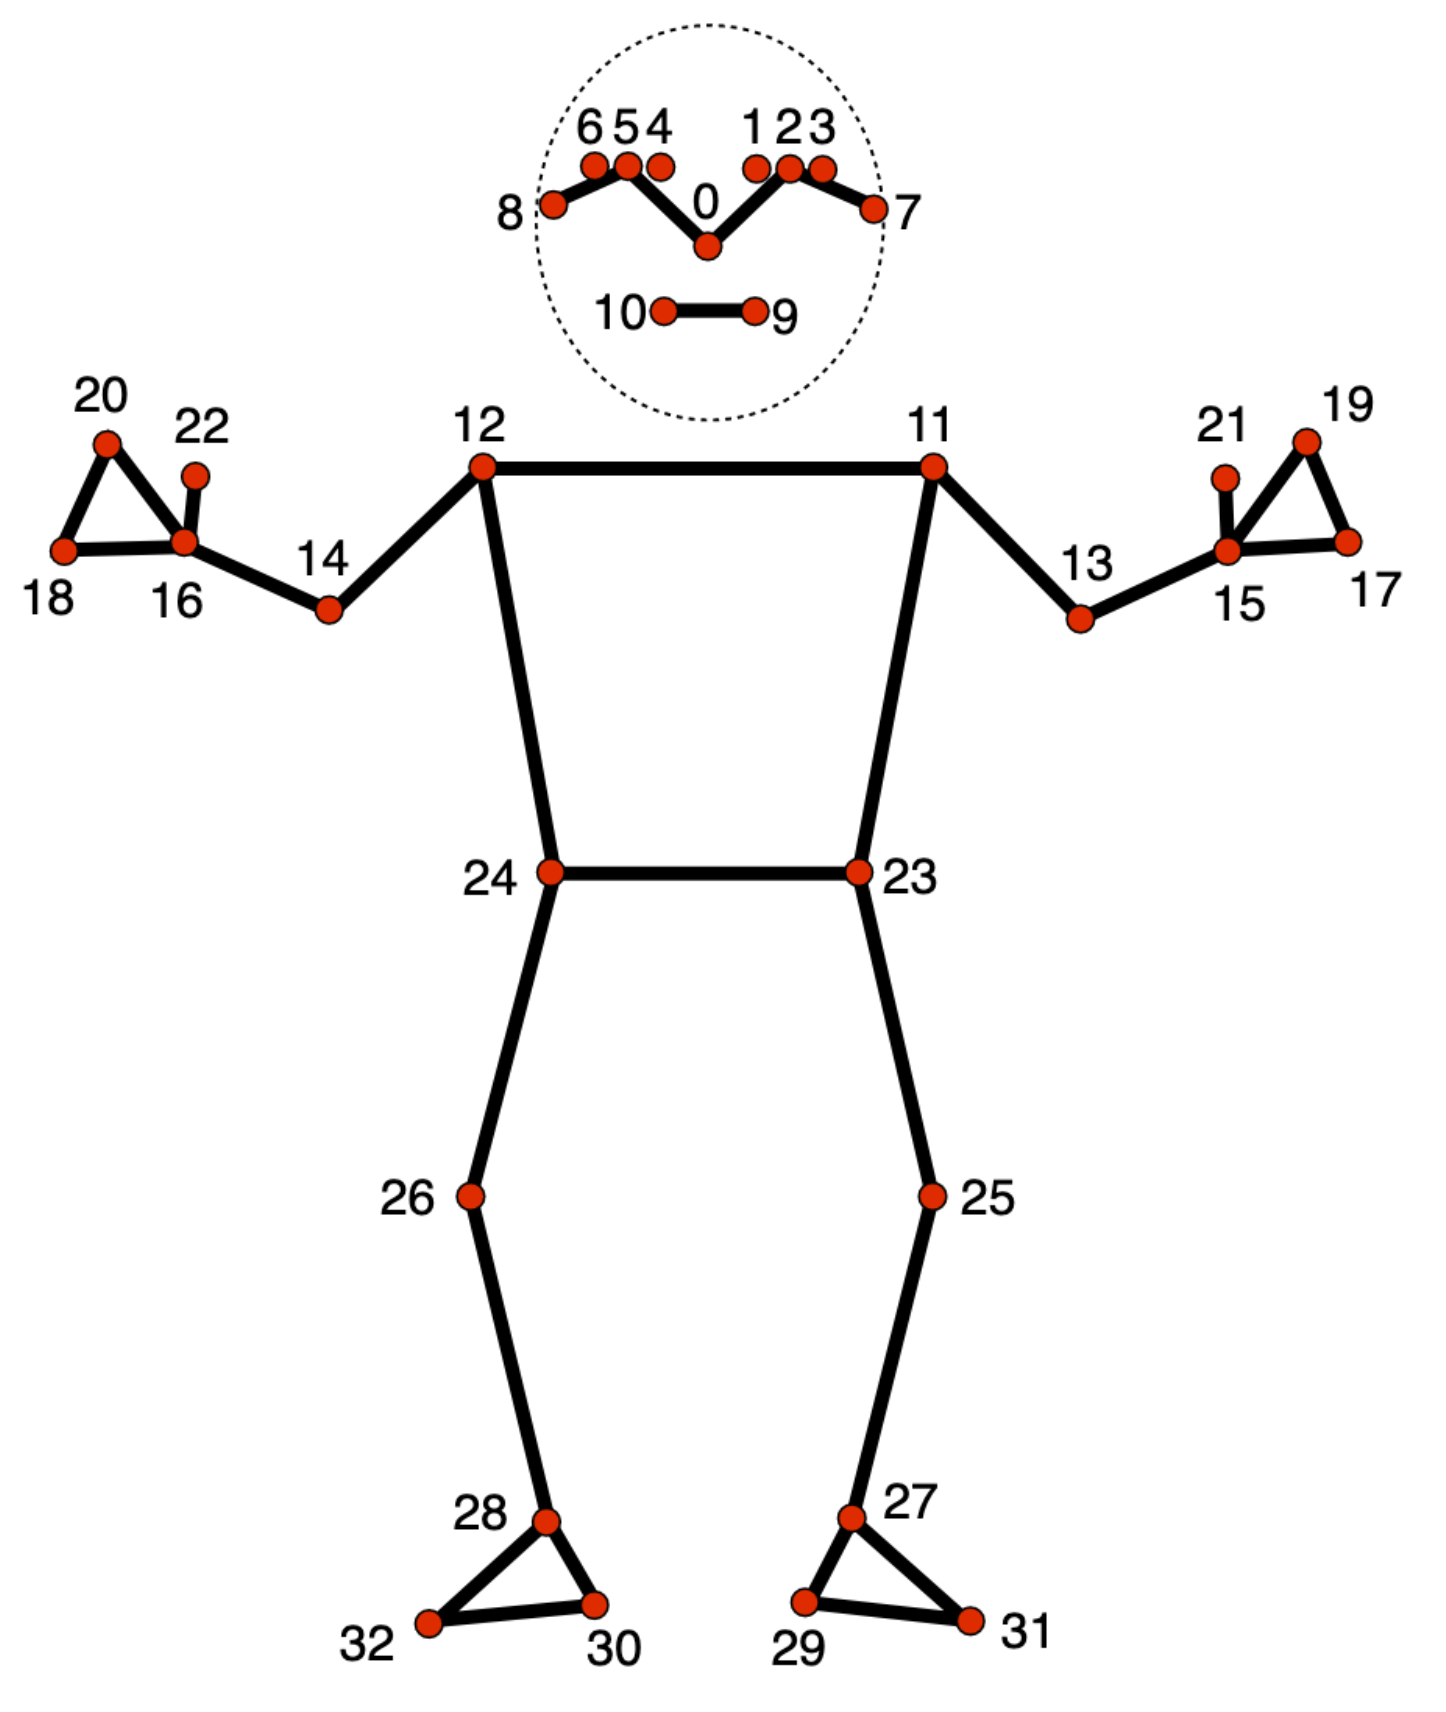
\includegraphics[scale=0.3]{figures/body_key_points.png}
    \caption[Set of detectable body key points]
    {Fixed set of detectable body key points offered by the mediapipe framework
    \cite{mediapipe_framework}}
    \label{fig:2_body_keypoints}
\end{figure}\\
Within this work, the key points in the head area (range [0 - 10]) are not of 
great interest apart from visualization purposes.\\
The knee, hip and arm key points however will be used for angle 
calculations and ground contact detection.
Thus, a good performance in detecting the according key points within these 
areas is crucial for the software's overall reliability.

\subsection{Why Mediapipe?}\label{subsec:2_why_mediapipe}
In recent years many approaches towards accurate body pose detection were 
developed and implemented.
Many of those offer decent accuracies, but often lack reasonable performance,
especially when no \ac{GPU} is available for hardware acceleration.
Following, two common alternatives to Mediapipe, namely OpenPose and AlphaPose,
are shortly presented and differentiated from the chosen Mediapipe framework.\\
One of the most widely used human pose detection libraries is the open source 
library \textit{OpenPose}.
As shown in~\cite{openPose} it offers a Multi-Person pose estimation that is 
especially useful when dealing with groups of people.
However, as this project is meant to be used for long jump evaluation, only one 
person needs to be tracked at a time.
Even though OpenPose of course can handle one person pose estimation, 
mediapipe outperforms OpenPose in this area.
Back in 2016 Kocabas et al.~achieved around 23~FPS using \ac{GPU} accelerated
OpenPose pose detection~\cite{openPose_speed_gpu} and Osokin later proposed an
improved neural network design, allowing for up to 28~FPS without hardware 
acceleration~\cite{openPose_speed_cpu}.
As of 2023 these benchmarks are still reasonable.
Mediapipe however achieves speeds of up to 63\% higher.\\
While OpenPose uses a \textit{Bottom-Up} approach due its multi-person 
application, Mediapipe uses the less computational complex \textit{Top-Down} 
approach.\\
Bottom-Up implementations first detect all body key points present in an input
image and then move on to grouping the recognized points in clusters.
Points in the same cluster are then assigned to one person.\\
Top-Down approaches however first roughly detect the overall body position 
within the input image and then define a region of interest\footnote{sometimes
also referred to as \textit{Bounding Box}} around the subject.
The following processing therefore only needs to take this defined region of 
interest into account, leading to significantly less computational complexity.\\
AlphaPose is another open source library often used for body pose estimation.
Just like OpenPose it uses a Bottom-Up approach to reliable offer multi-person
body pose detection.
Additionally, AlphaPose, like Mediapipe, offers multiple detection models that 
differ regarding accuracy and speed.
Again however, Mediapipe outperforms AlphaPose because of its Top-Down approach
and because AlphaPose is designed to work with \ac{GPU} acceleration, rather 
than running on \ac{CPU} only.\\
Another advantage of Mediapipe is its output.
While OpenPose and AlphaPose offer 2D coordinates for each detected key point,
Mediapipe additionally offers a depth estimation resulting in a spatial 3D 
coordinate for each detected key point.
Thereby, more comprehensive analysis can be performed.   

\subsection{OpenCV}\label{subsec:2_openCV}
OpenCV is an open source library commonly used for image processing in the 
area of computer vision and machine learning.
It is written in C++, thus offering high performance in numerical operations,
especially matrix operations.\\
\texttt{python-opencv} is the python wrapper for OpenCV which will be used in
this project to efficiently read and process video frames.
The python wrapper imports the underlying C++ functions as modules to take 
advantage of C++'s efficiency, resulting in significantly higher performance
compared to equivalent Python only implementations.
Furthermore, it is fully compatible with the \texttt{numpy} library, which 
allows for seamless conversion between numpy arrays and OpenCV image matrices.

\subsection{HDF5 file format}\label{subsec:2_hdf5}
After a jump analysis is completed, there are two files to be stored.
One video file containing the actual body key point video analysis by showing
the key points as overlay and another one holding the analyzed parameters.
The second file especially requires the file format to be structured in order
to be able to allocate the stored analysis parameters to their according video
frame.\\
One common open source structured file format is HDF5\cite{The_HDF_Group_Hierarchical_Data_Format}.
It is an acronym for Hierarchical Data Format (Version 5) and is very efficient 
to store large amounts of data as well as heterogeneous data.
As the name already suggests, data is stored in a hierarchical, tree-like way.\\
A HDF5 tree mainly consists of three pre-defined components that allow to 
organize data in a file-system like fashion.
Namely, those components are the tree root, groups and datasets.
\textit{Groups} are folder-like structures that can either contain more groups 
or Datasets.
\textit{Datasets} hold the actual data that need to be stored.\\
Furthermore, each level (tree root, groups and datasets) can hold additional 
information via metadata.
The metadata could, for example, contain information about metrics, timestamps or 
any other describing information.
Therefore, each HDF5 file itself becomes a self-describing file that does not
require any more than the included information to be interpreted correctly.\\
Thus, it is chosen as primary analysis parameter storage format within this
project.
\begin{figure}[!h]
    \centering
    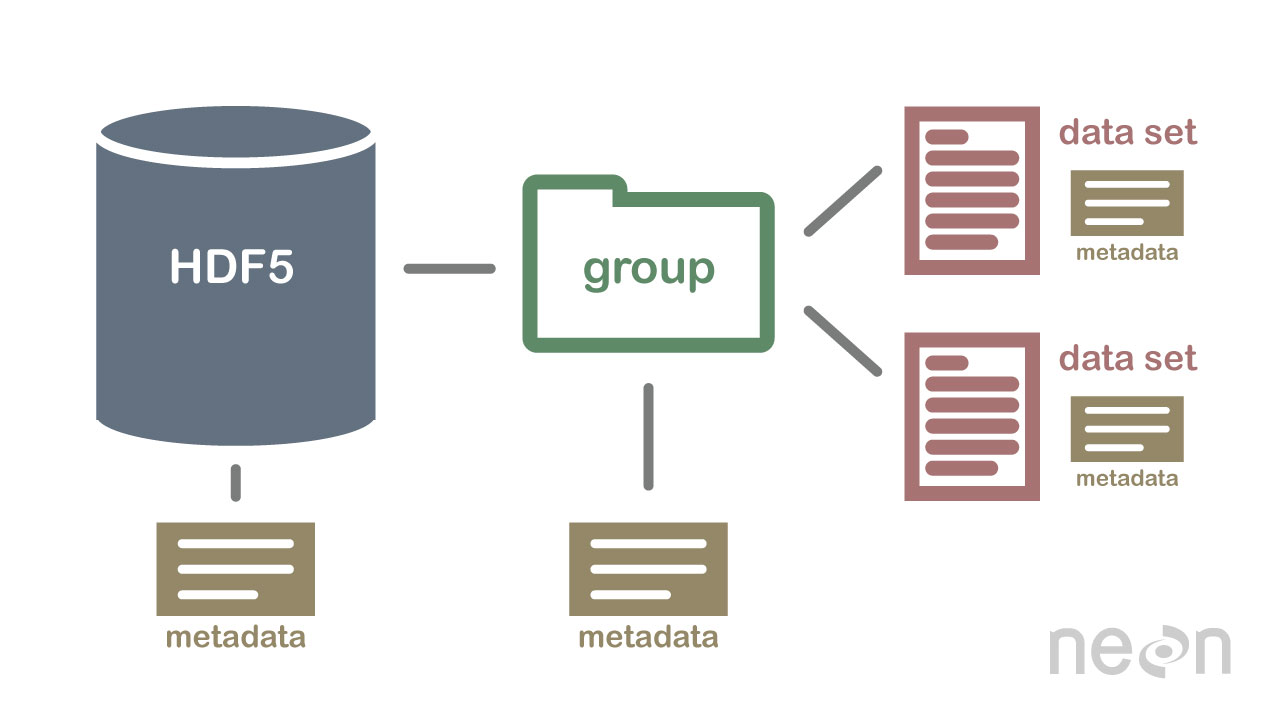
\includegraphics[scale=0.24]{figures/hdf5_general_structure.jpg}
    \caption[HDF5 file structure]
    {Principle HDF5 file structure~\footnote{
        \url{https://www.neonscience.org/resources/learning-hub/tutorials/about-hdf5}}}
    \label{fig:2_principle_hdf5_structure}
\end{figure}
\FloatBarrier
\noindent Within this work, one HDF5 file will be created per jump analysis.

\subsection{Precompiling Python code using Numba}\label{subsec:3_precompile_numba}
Built-in Python functions as well as some \texttt{numpy} functions can be
sped up using the Python \textit{Just-in-time compiler} \texttt{numba}
\cite{lamNumbaLLVMbasedPython2015}.
This compiler is based on the LLVM compiler structure and generates
\ac{CPU} specific, optimized machine code.
This is especially helpful in numerical heavy parts of the software, which can
significantly benefit from pre-compiled code regarding their runtime behavior.

\subsection{Software overview}\label{subsec:3_versions}
The software within this work is implemented using python (see
\autoref{subsec:2_programming_language}).
As it supports a wide range of software features, a variety of
different packages is used.
The most relevant packages and frameworks are numpy for efficient numerical
operations, h5py for convenient HDF5 file operations and PyQt5, which is used
for the \ac{GUI} development.\\
Moreover, the software has been implemented and tested using Python
3.11.5 and is backward compatible up to Python 3.9.
Python 3.12 is explicitly not supported, as the mediapipe framework not yet
supports this version.
As the packages are combined into one software, an overview of the used
packages is given:

\begin{table}[h!]
    \centering
    \begin{tabular}[c]{|p{6cm}|p{6cm}|}
    \hline
    \multicolumn{2}{|c|}{\cellcolor{gray!20}Software package overview}\\
    \hline
    Package & Version number\\
    \hline
    \hline
    \multicolumn{2}{|c|}{\cellcolor{cyan!15}Jump analysis}\\
    \hline
    mediapipe & 0.10.7\\
    \hline
    numpy & 1.26.1\\
    \hline
    numba & 0.59.0\\
    \hline
    scipy & 1.12.0\\
    \hline
    opencv-python & 4.8.1.78\\
    \hline
    psutil & 5.9.6\\ 
    \hline
    h5py & 3.10.0\\
    \hline
    \multicolumn{2}{|c|}{\cellcolor{cyan!15}\acs*{GUI} development}\\
    \hline
    PyQt5 & 5.15.10\\
    \hline
    PythonQwt & 0.11.1\\
    \hline
    \multicolumn{2}{|c|}{\cellcolor{cyan!15}Drone control}\\
    \hline
    pymavlink & 2.4.41\\
    \hline
    pyserial & 3.5\\
    \hline
    \end{tabular}
    \caption[Software overview]{Software package overview and their according
    version numbers.}
    \label{table:3_software_overview_version_num}
\end{table}
\FloatBarrier

%TODO: related work

\section{\acs*{GUI} development}
The software that is developed within this work should be useable on-field to
allow for a fast analysis process.
Besides the video analysis, the drone control should be embedded in the same 
software to always guarantee control over the drone.\\
Thus, a simple \ac{GUI} is developed to offer a convenient drone control and 
video analysis process.\\
The \ac{GUI} is developed using Qt and its Python binding PyQt.
Both are presented in this section. 

\subsection{Development framework Qt}\label{subsec:2_qt}
Qt is a development framework based on the programming language C++.
It includes a \ac{GUI} toolkit and therefore enables platform-independent
application development.
All common platforms including Linux, Windows and MacOS are supported by 
Qt.
Additionally, both mobile operating systems, Android and iOS, are supported.\\
This project however will focus on the development of an application that is 
able to run under Windows, Linux and MacOS.\\
The Qt framework is mainly chosen because of its rich and comprehensive 
documentation\footnote{\url{https://doc.qt.io/}} and the availability of the 
well-supported Python binding \textit{PyQt}.\\
As Qt is based on C++ all Qt source files are translated to C++ code.
This step is realized by the \texttt{Meta Obejet Compiler (MOC)} which is 
integrated as pre-processor.
Thus, all Qt files are translated to so-called \textit{Meta Obejet Code}, 
which can be seen as C++ source code with some enhancements.
The most important enhancement is the signal and slot functionality which 
allows for an easy communication between different software and design 
elements (e.g.\ show a message dialog when a button is clicked).\\
Another important enhancement for this work is the convenient multi-threading
management necessary for offering a responsive \ac{GUI} even when cpu-bound 
calculations such as image processing is performed.

\subsection*{The \acs*{GUI} module PyQt}\label{subsec:2_pyqt}
The discrepancy between Qt as C++ based framework and Python as chosen
programming language for this project (as explained in \autoref{subsec:2_programming_language})
can be overcome using Qt's Python binding PyQt.
By using PyQt we can combine Python's machine learning advantages with Qt's 
platform-independent \ac{GUI} development.
More specifically \textit{PyQt5} \footnote{\url{https://pypi.org/project/PyQt5/}} 
is used.\\
It allows building complex Qt applications using Python only instead of C++.
All other described advantages that Qt offer remain valid despite the use 
of PyQt.
Thus, the whole software within this project including the \ac{GUI} can be 
developed using Python as programming language.
    \graphicspath{{./figures/}}
\chapter{Implementation}
This chapter focuses on the overall project's implementation.
It mainly covers the four parts hardware assembly, long jump analysis,
drone control and their consolidation into one \ac{GUI}.

\section{Long-jump analysis software}\label{sec:4_analysis_software}
In order to analyze recorded long jump videos a ground station software is
developed.
Generally, the analysis is performed regarding the following set of
parameters:
\begin{itemize}
    \item left / right knee angle
    \item left / right arm angle
    \item takeoff angle
    \item left / right foot position
    \item hip height
\end{itemize}
These parameters are tracked over the whole jump, beginning with the run-up
throughout the takeoff until the landing.\\
\autoref{fig:4_long_jump_sketch} shows a detailed overview over the video data
that can be analyzed by the software.\\
As the takeoff is (one of) the most important phases in a long jump, it is
important to be able to detect the takeoff in a video.
Such a takeoff detection is developed alongside the above-mentioned parameter 
detection- and calculation.\\
This section will first introduce the body key point detection process that
is basis for all following calculations.
Afterwards, an algorithm for an automatic takeoff frame detection based on a
video input is implemented.
\begin{figure}[!h]
    \centering
    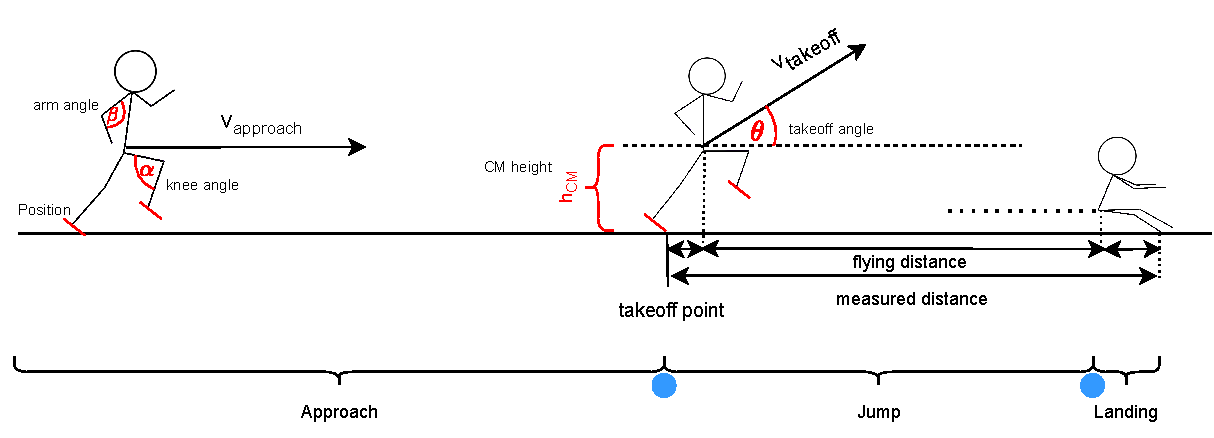
\includegraphics[scale=0.6]{long_jump_sketch.pdf}
    \caption[Long jump parameter overview]{General overview of the parameters
    that are important in a long jump.\\
    Parameters that can be analyzed by the software are marked
    \textcolor{red}{red}.\\
    The \textcolor{cyan}{blue points} indicate phase transition points.}
    \label{fig:4_long_jump_sketch}
\end{figure}
\FloatBarrier

\subsection{Detecting body key points}\label{subsec:4_body_keypoint_detection}

\subsection{Calculating analysis parameters}\label{subsec:4_calc_params}

\subsection{Automatic takeoff frame detection}\label{subsec:4_takeoff_detection}
Generally, a long jump can be divided into three different phases, namely
approach, jump and landing.
In \autoref{fig:4_long_jump_sketch} an overview over the phases is given,
where the takeoff phase is represented by the first phase changing point.\\
Each phase demands different requirements from an athlete, however, the
takeoff phase is the last phase in which an athlete is able to actively
influence the most important jumping conditions.
Within this short\footnote{0.1s \- 0.2s\cite{mechanical_power_long_jump}} time
period the initial kinetic run-up energy is transformed into jumping energy.
Especially the velocity vector of an athletes' \ac{CM} changes its direction
in the moment of the takeoff, as illustrated in
\autoref{fig:4_long_jump_sketch}.
The forces produced during the takeoff strongly influence the resulting
jumping distance. 
Thus, it is important to understand its dynamics.\\
Due to the short time period a takeoff takes, it can be difficult to detect
the takeoff frame in a long jump video in order to be able to analyze the
exact pre-jump conditions.\\\\
However, especially to allow for an on-field jumping analysis, a quick takeoff
frame detection is crucial.
Thus, an algorithm that can automatically detect the takeoff frame in a long
jump video is implemented in the following.\\\\
As the automatic takeoff frame detection is based on the parameters listed in
\autoref{sec:4_analysis_software}, the left and right
foot position as well as the position of the \ac{CM} were analyzed in
pre-recorded long jump videos of male long jumpers at different professional
levels reaching from hobby- to olympian athlete.
Moreover, the videos used differ in their length and quality as well as in the
jumping part they show (e.g.\ video 2 does not show the full run-up).
The results of three exemplary video analysis are shown in
\autoref{fig:4_angles_height_plot}.
In order to develop an accurate takeoff point detection, the takeoff frame was
first manually selected (marked as \textcolor{blue}{blue vertical line} for
each analysis in \autoref{fig:4_angles_height_plot}).\\
The presented data has not been cleaned up in any way.
This can especially be seen in the first and last analysis, in which the
position and angle data is not accurate due to body key point detection
inaccuracies.
These inaccuracies however are not of great interest as the key points are
detected correctly during the approach after a few frames.\\\\
In each analysis the left and right foot positions as well as the
according knee angles interchange from step to step.
The relative \ac{CM} height remains on the same level during the approach.\\
Behind the takeoff point, the relative hip- and foot heights increase quickly
until the maximal height is reached and the landing phase starts.
Moreover, the swing legs' foot height increases faster in comparison to the
jumping legs' foot height as the latter one stays on the ground longer to
introduce the jump.\\
In the moment of the takeoff, the knee angle of the jumping leg is above 170
degree, meaning the jumping leg is fully extended.
The swing legs' knee angle varies in the shown examples around 100 degree.\\\\
The visually most significant change which happens in the moment of the
takeoff and is therefore the most meaningful measured parameter that indicates
the takeoff is the change of height of the \ac{CM}.
Thus, the automatic takeoff detection is developed based on this parameter.\\
To approach the detection of the rapid change in the \ac{CM}s' vertical
velocity, a mathematical description of its position during the jump is
modelled.

\begin{figure}[h!]
    \begin{subfigure}[b]{0.5\textwidth}
        \includegraphics*[scale=0.45]{jump_runup_poor_start.png}
        \captionsetup{justification=centering, singlelinecheck=false, labelfont=bf}
        \label{subfig:runup_jump_landing_height}
    \end{subfigure}
    \begin{subfigure}[b]{0.5\textwidth}
        \includegraphics*[scale=0.45]{jump_runup_poor_start_angles.png}
        \label{subfig:runup_jump_landing_angles}
    \end{subfigure}
    \begin{subfigure}[b]{0.5\textwidth}
        \includegraphics*[scale=0.45]{jump_no_runup.png}
        \label{subfig:no_runup_height}
    \end{subfigure}
    \hfill
    \begin{subfigure}[b]{0.5\textwidth}
        \includegraphics*[scale=0.45]{jump_no_runup_angles.png}
        \label{subfig:no_runup_angles}
    \end{subfigure}
    \begin{subfigure}[b]{0.5\textwidth}
        \includegraphics*[scale=0.45]{jump_runup_poor.png}
        \label{subfig:runup_jump_height}
    \end{subfigure}
    \begin{subfigure}[b]{0.5\textwidth}
        \includegraphics*[scale=0.45]{jump_runup_poor_angles.png}
        \label{subfig:runup_jump_angles}
    \end{subfigure}
    \caption[Analyzed jumping parameters over time]{Analyzed and calculated
    jumping parameters over time.\\
    \textbf{Left column}: Analyzed left / right foot height and hip height.\\
    \textbf{Right column}: Calculated knee angles over time.\\
    The \textcolor{blue}{vertical lines} represent the visually selected
    takeoff point.\\
    \textbf{First row}: full run-up, full jump. \textbf{Second Row}: short 
    run-up, full jump.
    \textbf{Third row}: full run-up, full jump, poor video quality}
    \label{fig:4_angles_height_plot}
\end{figure}
\FloatBarrier

\subsubsection{Regression}
As the takeoff point detection is based on linear and quadratic regression,
both are briefly introduced in the following.
Regression generally describes the approximation of a polynomial function to
fit a given dataset.
The dataset that is tried to be approximated in this case is the height of the
\ac{CM}.
The dataset can be expressed as (T, H), where H holds the heights of the
\ac{CM} and T holds the related time points.
As the input is a video, T represents a simple vector holding the
video's frame numbers.
For the following steps it is helpful to express T and H as column vectors:
\begin{equation}
    \vec{t} = \begin{bmatrix}
        1\\
        2\\
        \vdots\\
        n
    \end{bmatrix}
        \quad\text{and}\quad
    \vec{h} = \begin{bmatrix}
        h_1\\
        h_2\\
        \vdots\\
        h_n
    \end{bmatrix}
\end{equation}
where n is the total number of video frames and $h_i$ is the $i\--th$ recorded
height of the \ac{CM}.\\
Taking the \ac{CM} in \autoref{fig:4_angles_height_plot} into consideration,
a whole jump can hardly be fitted with a single polynomial function.
However, as shown in \autoref{fig:4_long_jump_sketch}, a long jump consists of
multiple phases.\\
This offers an opportunity to detect the takeoff.
As mentioned before, the takeoff frame is defined as the point where the
approach phase ends and the jumping phase starts, ($PT_0$ in
\autoref{fig:4_long_jump_sketch}).
Thus, if a mathematical expression can be found for each phase respectively,
the takeoff frame is found implicitly.\\
The runup phase includes all frames in the interval $[0, PT_0[$, the jumping
phase is covered by the frames in range $[PT_0, PT_1[$ and the landing phase
is shown by the frames in the interval $[PT_1, n[$, where $PT_0$ defines the
first Phase Transition point (the takeoff) and $PT_1$ the point at which the
landing phase starts.
Each phase by itself can be approximated with a polynomial function.
The approach and the landing can be fitted using a linear expression.\\
Thus, two linear regressions are performed separately to find two expressions
of the form
\begin{equation}\label{eq:linear_function}
    \\y_i = \beta_0 + \beta_1t_i + \epsilon_i
    \quad\quad
    i = \text{start},\ \dots\ ,\text{end}
\end{equation}
where $\beta_0$ and $\beta_1$ are the coefficients that need to be found.
start and end represent the first and last frame index that should be
considered in the linear regression.
For the approach phase this leads to $start = 0$ and $end = TP_0 - 1$, the
landing phase is accordingly represented by $start = TP_1$ and $end = n - 1$.\\
\autoref{eq:linear_function} can also be expressed as matrix equation:
\begin{equation}\label{eq:linear_reg_matrix}
    \underbrace{
    \begin{bmatrix}
        y_0\\
        y_1\\
        \vdots\\
        y_r\\
    \end{bmatrix}}_{\substack{\vec{y}}}
    =
    \underbrace{
    \begin{bmatrix}
        1 & t_{\text{start}}\\
        1 & t_{\text{start} + 1}\\
        \vdots & \vdots\\
        1 & t_{\text{end}}
    \end{bmatrix}}_{\substack{\text{Design matrix} \\ T}}
    \underbrace{
    \begin{bmatrix}
        \beta_0\\
        \beta_1
    \end{bmatrix}}_{\substack{\text{Coefficients} \\ \text{vector} \\
    \vec{\beta}}}
    +
    \underbrace{
    \begin{bmatrix}
        \epsilon_0\\
        \epsilon_1
    \end{bmatrix}}_{\substack{\text{Error} \\ \text{vector} \\
    \vec{\epsilon}}}
\end{equation}
where $r = end - start$.
This can be written in short form as:
\[
    \vec{y} = T\vec{\beta} + \vec{\epsilon}    
\]
Now, the vector $\vec{\beta}$ needs to be found that minimizes the sum of
errors $E_{SSE}$ between the measured \ac{CM} height $h_i \in \vec{h}$ and the
fitted polynomial $y_i$ at time step i.
To measure the error, the \ac{SSE} is used:
\begin{equation}
    E_{SSE} = \sum_{i=start}^{end} \epsilon_i^2 = \sum_{i=start}^{end} (h_i - y_i)^2
\end{equation}
Using the simple linear expression from \autoref{eq:linear_function},
following error function is found:
\begin{equation}
    E_{SSE} = \sum_{i=start}^{end} (h_i - \beta_0 - \beta_1i)^2
\end{equation}
By using the matrix notation introduced in \autoref{eq:linear_reg_matrix},
the equation above can be written in matrix notation as well:
\begin{equation}\label{eq:sse_matrix}
    E_{SSE} = (T\vec{\beta} - \vec{h})^T(T\vec{\beta} - \vec{h})
\end{equation}
As $\vec{\beta}$ should minimize $E_{SSE}$, the minimum of $E_{SSE}$ is
needed, which can be found by solving following equation:
\begin{equation}\label{eq:gradient_linear_case}
    \nabla_{\vec{\beta}}E_{SSE} = \nabla_{\vec{\beta}}(T\vec{\beta} - \vec{h})^T(T\vec{\beta} - \vec{h}) = 0
\end{equation}
where $\nabla_{\vec{\beta}}$ denotes the gradient with respect to $\vec{\beta}$.\\
The coefficients can then easily be found by solving
\autoref{eq:gradient_linear_case} for $\vec{\beta}$, which yields the 
following normal equation:
\begin{equation}\label{eq:normal_equation}
    \vec{\beta} = (T^T T)^{-1}(T^T\vec{h})
\end{equation}
that especially requires $(T^{T} T)$ to be invertible.
A proof of \autoref{eq:normal_equation} can be found in
\cite{proof_linear_regression_mat}.\\
As mentioned, this process is performed twice to find a linear approximation
for the approach and the landing phase of an athletes' \ac{CM} respectively.\\\\
The jumping phase cannot be approximated with a linear polynomial.
However, as can be seen in \autoref{fig:4_angles_height_plot} after the marked
takeoff point, the curve of the \ac{CM} height can be approximated using a
parabola.
Thus, quadratic regression is used to find a curve that describes the height
of the \ac{CM} during the jumping phase.
The second order polynomial that needs to be found is of the form:
\begin{equation}\label{eq:quadratic_function}
    \\y_i = \beta_0 + \beta_1t_i + \beta_2t_i^2 + \epsilon_i
    \quad\quad
    i = PT_0,\ \dots\ ,PT_1 - 1
\end{equation}
$PT_0\ \text{and}\ PT_1$ are the phase transition points shown in
\autoref{fig:4_long_jump_sketch}.
The following steps are equal to the linear regression shown above.
Thus, only the differences are shown in detail.\\
The T matrix in \autoref{eq:linear_reg_matrix} contains all frame
numbers as column vector.
Because a linear relation was tried to be found to approximate the approach
and  landing phase before, the T matrix as well only contained linear values.
Now however, a quadratic relation needs to be found.
Thus, the T matrix needs to be extended by one more column holding the
quadratic frame numbers yielding following matrix equation:
\begin{equation}\label{eq:quadratic_reg_matrix}
    \underbrace{
    \begin{bmatrix}
        y_0\\
        y_1\\
        \vdots\\
        y_r\\
    \end{bmatrix}}_{\vec{y}}
    =
    \underbrace{
    \begin{bmatrix}
        1 & t_{PT_0} & t_{PT_0}^2\\
        1 & t_{PT_0 + 1} & t_{PT_0 + 1}^2\\
        \vdots & \vdots & \vdots\\
        1 & t_{PT_1 - 1} & t_{PT_1 - 1}^2
    \end{bmatrix}}_{T}
    \underbrace{
    \begin{bmatrix}
        \beta_0\\
        \beta_1\\
        \beta_2
    \end{bmatrix}}_{\vec{\beta}}
    +
    \underbrace{
    \begin{bmatrix}
        \epsilon_0\\
        \epsilon_1\\
        \epsilon_2
    \end{bmatrix}}_{\vec{\epsilon}}
\end{equation}
where $r = PT_1 - 1 - PT_0$.
The error function which needs to be minimized can be set equivalent to the
linear case (\autoref{eq:sse_matrix}).
Comparing \autoref{eq:linear_reg_matrix} and \autoref{eq:quadratic_reg_matrix}
the only things that change are the number of coefficients (and thus the
number of error terms) as well as the design matrix T, which holds one more
column.
The steps to determine the coefficients $\vec{\beta}$ are equal to the linear
case in equations~\ref{eq:sse_matrix} to~\ref{eq:normal_equation}.
$\vec{\beta}$ is then given by the same normal equation~
\ref{eq:normal_equation} as in the linear case:
\[
    \vec{\beta} = (T^T T)^{-1}(T^T\vec{h}) 
\] 
where $\vec{\beta}$ contains three coefficients $\beta_0$, $\beta_1$ and
$\beta_2$ to approximate the jumping phase.\\\\

\noindent By using this linear- and quadratic regression approach, the whole
jump can be modelled mathematically.
However, in order to find the best fitting model, the phase changing points
($PT_0$ and $PT_1$ in \autoref{fig:4_long_jump_sketch}) need to be determined.
This can be done by minimizing the overall error $E_{total}$, which is defined
as the sum of regression errors resulting from the three independent
regressions performed (one per jumping phase):

\begin{equation}
    E_{total} = E_{approach} + E_{jump} + E_{landing}
\end{equation}

\noindent $E_{total}$ can be minimized by using a brute-force approach.
For each possible combination of phase transition points, two linear
regressions (representing approach and landing) and one quadratic regression
(representing the jumping phase) are performed and their individual errors
given by \autoref{eq:sse_matrix} are summed up.
The combination of phase transition points that leads to the minimal
$E_{total}$ is then considered as the optimal model to fit the overall jump.
As the found phase transition points directly represent their corresponding
frame numbers, the takeoff frame is directly given by the first phase
transition point.\\

\begin{figure}[htp]% [H] is so declass\'e!
    \centering
    \begin{minipage}{0.45\textwidth}
    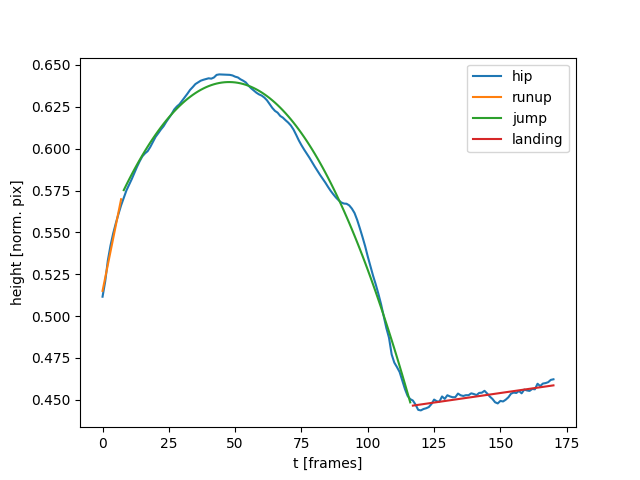
\includegraphics[width=\textwidth]{regression_jump_only.png}
    \caption{figure caption}
    \end{minipage}\hfill
    \begin{minipage}{0.45\textwidth}
    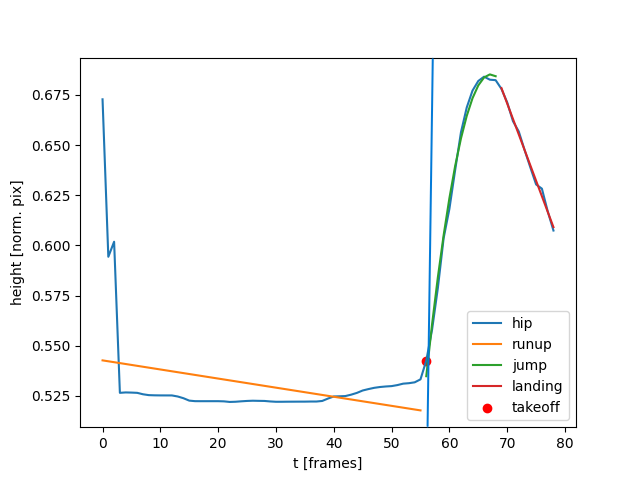
\includegraphics[width=\textwidth]{regression_poor_approach.png}
    \caption{figure caption}
    \end{minipage}\par
    \vskip\floatsep% normal separation between figures
    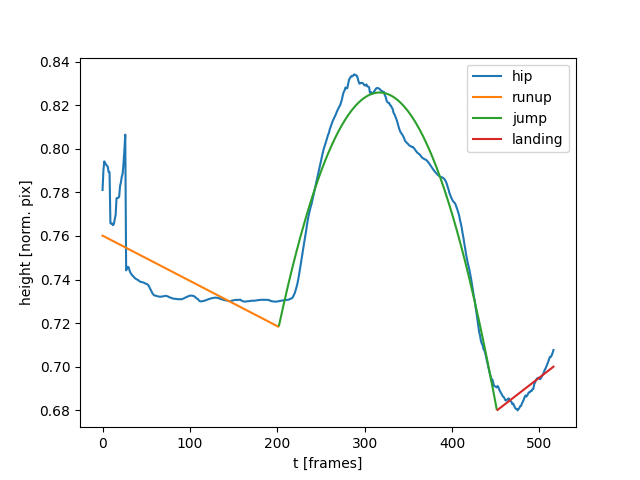
\includegraphics[width=0.45\textwidth]{regression_poor_approach_jump.png}
    \caption{figure caption}
    \end{figure}
\FloatBarrier

\begin{algorithm}
    \caption{takeoff\_frame(hip\_height: array)}
    \begin{algorithmic}[1]
    \State $n \gets \text{length of } hip\_height$
    \State $total\_error \gets 100$
    \State $changing\_points \gets (0,0)$
    \State $runup\_coeffs \gets []$
    \State $jump\_coeffs \gets []$
    \For{$i \gets 0$ \textbf{to} $n - 2$}
        \For{$j \gets i + 2$ \textbf{to} $n$}
            \State $x\_runup \gets \text{array of } i \text{ elements from } 0 \text{ to } i - 1$
            \State $x\_jump \gets \text{array of } (j - i) \text{ elements from } 0 \text{ to } j - i - 1$
            \State $x\_landing \gets \text{array of } (n - j) \text{ elements from } 0 \text{ to } n - j - 1$
            \State $hip\_fit\_runup, residuals\_runup \gets \text{polyfit}(x\_runup, hip\_height[:i], 1)$
            \State $hip\_fit\_jump, residuals\_jump \gets \text{polyfit}(x\_jump, hip\_height[i:j], 2)$
            \State $hip\_fit\_landing, residuals\_landing \gets \text{polyfit}(x\_landing, hip\_height[j:], 1)$
            \State $fitting\_error \gets residuals\_runup + residuals\_jump + residuals\_landing$
            \If{fitting\_error $<$ total\_error \textbf{and} hip\_fit\_jump[0] $<$ 0}
                \State $total\_error \gets$ fitting\_error
                \State $changing\_points \gets (i,j)$
                \State $runup\_coeffs \gets hip\_fit\_runup$
                \State $jump\_coeffs \gets hip\_fit\_jump$
            \EndIf
        \EndFor
    \EndFor
    \State \textbf{return} changing\_points
    \end{algorithmic}
    \end{algorithm}

\section{Hardware setup}\label{sec:4_hardware}
In order to capture high-quality video recordings that cover a complete long 
jump, from the first step all the way to the landing, a drone is used to fly
next to the athlete throughout the whole process.
Thus, a drone in form of a quadcopter is built from scratch.
Its control will be integrated seamlessly in the projects' \ac{GUI}.\\
This section introduces the hardware components that are used for building 
this drone as well as its flight control unit.\\
A short outline of the hardware is given in 
\autoref{subsec:4_hardware_selection},
while \autoref{subsec:4_hw_setup} focuses on the overall assembly of the 
selected hardware.

\subsection{Hardware selection}\label{subsec:4_hardware_selection}
Currently, commercial drone hardware on the market is mainly separable into 
the two large areas of fully remote controlled \ac{FPV} hardware and hardware 
for (autonomous) drones that can usually carry more load, e.g.~heavy cameras.
Even though the quadcopter in this project needs to be remotely 
controllable from a ground station pc, it is still more likely to be located 
in the latter one.\\
Generally the hardware was chosen based on the following criteria:
\begin{itemize}
    \item price
    \item compatibility
    \item size
\end{itemize}

\subsection*{Flight Hardware}\label{subsec:4_filght_hardware}
The main hardware that a quadcopter needs to fly will, in the following, be
referred to as \textit{flight hardware}.
This includes frame, motors, rotors, \acp{ESC} and a \ac{PDB}.\\
The main platform on which all drone hardware is mounted, is referred to as
a quadcopter's frame.
As this project's drone does not need to carry any heavy load, such as high 
precision camera systems or other sensors, a rather compact frame would 
theoretically be sufficient.
However, compact frames tend to be less stable compared to larger frame sizes 
which could lead to a lower video recording quality and thus require more 
complex post-processing software.
Moreover, the assembly process on larger frames is more convenient and 
replacing parts is easier.
Additionally, compact frames are most commonly used in areas that demand quick
reaction times for high speed flight maneuvers, e.g.~in drone racing.
This however is not needed in this project's context.\\
Taken the mentioned considerations into account the mid-sizes \textit{Holybro 
S500 V2} frame kit is chosen.
Besides the frame, the kit also includes a landing gear and rotors.
Moreover, the main platform includes a \ac{PDB} to split the battery's power 
equally to all four motors.\\
An overview of all included parts is given in \autoref{fig:4_frame_kit}.
\begin{figure}[!h]
    \centering
    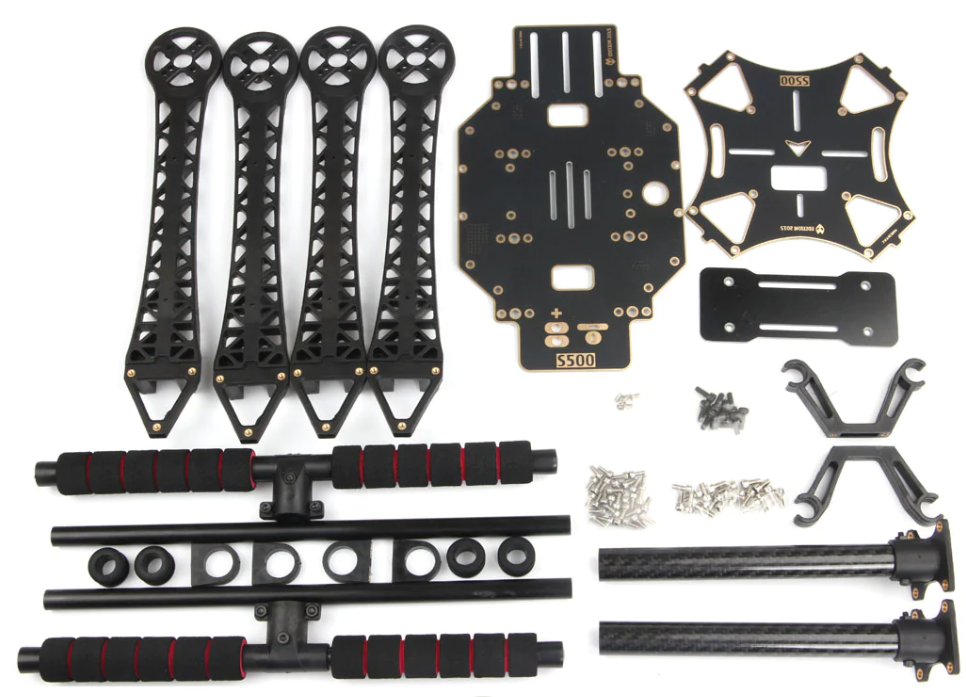
\includegraphics[scale=0.6]{frame-kit.png}
    \caption[Frame kit]{Holybro S500 V2 frame kit}
    \label{fig:4_frame_kit}
\end{figure}
\FloatBarrier
\noindent Besides the frame, motors and compatible \acp{ESC} are crucial 
flight hardware components.
Each motor requires an own \ac{ESC} that translates signals from a flight 
control unit to a voltage and thereby control the motors' rotation speed.
To guarantee compatibility, both components were chosen from Holybro as well
and can be seen in \autoref{fig:motors_and_esc}.
\begin{figure}[!h]
    \begin{subfigure}[b]{0.48\textwidth}
        \includegraphics*[scale=0.15]{motor.jpg}
        \caption{920KV Motor}
        \label{subfig:motor_picture}
    \end{subfigure}
    \hfill
    \begin{subfigure}[b]{0.5\textwidth}
        \includegraphics*[scale=0.15]{esc.jpg}
        \caption{\acl*{ESC}}
        \label{subfig:esc_picture}
    \end{subfigure}
    \caption[Motor and \acs*{ESC}]{Motor (a) and \acs*{ESC} (b)}
    \label{fig:motors_and_esc}
\end{figure}
\FloatBarrier
The drones' motors performance capabilities are defined by the number of 
\ac{RPM} they can perform per 1V input.
As can be seen in \autoref{subfig:motor_picture}, this link between 
rotation speed and input voltage is expressed in the arbitrary unit \textit{KV}.
The chosen motors are capable of rotating with a speed of 920~\ac{RPM} per 1V 
input voltage. 
Put into context, this is a common rotation speed in commercial and hobby 
drone applications.
Racing drones however, operate at motor speeds of up to 3500~KV.

\subsection*{Control Hardware}\label{subsec:4_control_hardware}
In order to perform flight maneuvers with a quadcopter, each motor must be
controllable individually.
The calculation of the correct rotation speeds is generally performed by 
a \textit{flight control unit}.
Usually, it receives directional instructions from a remote control as input,
combines them with many parameters (e.g.~\acs{GPS} position, height over ground,
speed, etc.) and generates a (\acs{PWM}) output signal for each motor.\\
Within this project the flight controller needs to deal with two different 
inputs.
First, the ground station which can be seen as a remote control in this case.
Additionally, the drone should be able to fly autonomously next to an athlete
during their long jump training.
Here, the second input gets important.
The autonomous fly option requires the quadcopter to perform a person 
detection and therefore image processing on-board.
As the flight controller itself is not able to perform such calculations, an
additional \textit{companion computer} is required.
This companion computer will then send directional instructions just like the 
ones from the ground station to the flight controller and thereby control the 
drone.\\
The combination of flight controller and on-board companion computer will in 
the following be called \textit{control hardware}.\\
There are many types of different flight controllers available commercially.
However, most of them are not meant to be used in combination with a companion
computer.\\
Two of the most commonly used flight controllers in autonomous drone projects
are the \textit{PixHawk} and the \textit{Navio2}.
They are often chosen because they both work together seamlessly with a 
companion computer.
The former is a totally independent system which can also operate without any 
supporting computer.
The latter is implemented as \ac{HAT} specifically designed for a Raspberry 
Pi.
Thus, it does not include an own \ac{CPU} but uses the Raspberry Pis's 
resources to perform flight relevant calculations.\\
A detailed comparison between both flight controllers is given in 
\autoref{table:4_flight_cotroller_cmp}.
\begin{table}[h!]
\centering
\begin{tabular}[c]{|p{4cm}||p{4cm}|p{4cm}|}
\hline
\multicolumn{3}{|c|}{Flight Controller Comparison}\\
\hline
Criteria & PixHawk & Navio2\\
\hline
\hline
Processor & ARM Cortex M4 with FPU / 32-bit co-processor & Depends on Raspberry
Pi version\\
\hline
Sensors & ST Micro 16-bti gyroscope, ST Micro 14-bit accelerometer, MEAS
barometer & MPU9250 9DOF IMU, LSM9DS1 9DOF IMU, MS5611 Barometer, U-blox M8N 
Glonass/\acs{GPS}/Beidou\\
\hline
Interfaces & UART, Spektrum DSM, PPM / S.BUS input, I2C, SPI, CAN, USB, 3.3V 
and 6.6V ADC input, 8 \acs{PWM} outputs, 6 Auxiliary outputs & UART, I2C, ADC, PPM / 
S.BUS input, 14 \acs{PWM} outputs\\
\hline
Dimensions\newline(W x H x L) in mm & $50 \times 15.5 \times 81.5$ & $55 \times 65$\\ 
\hline
Other & Failsafe options (e.g. extra power supply, \acs{GPS}, etc.) & None\\
\hline
Price (Eur.) & TBD & TBD\\
\hline
\end{tabular}
\caption[Flight controller comparison]{Comparison between PixHawk and 
Navio2 flight controller.}
\label{table:4_flight_cotroller_cmp}
\end{table}

\noindent As can be seen, both flight controllers offer different interfaces 
to connect additional hardware.
Moreover, both systems include sensors, mostly to gather information about 
drone's current position and inertia.
Here, the Navio2 even offers more sensors, as it already includes a \ac{GPS} 
sensor, while the PixHawk relies on an external one.\\\\
\noindent For this project, the PixHawk was chosen over the Navio2 mainly for 
three reasons.
First, it is on the market for a long time already and thus have a large 
community support.
Secondly, as it is an independent system, a failure of the companion computer 
will not lead to a crash.
Lastly, it allows for a wide range of companion computers, while the Navio2 
can only interoperate with a Raspberry Pi.\\
Furthermore, the mentioned considerations lead to easy rapid prototyping 
approaches, as the drone can be manually flown without a companion computer in
a first implementation.

\subsection{Hardware assembly}\label{subsec:4_hw_setup}
In the following, a high-level overview of the quadcopters' hardware setup is 
given.
The general wiring is shown and explained before a short introduction of some 
important communication protocols is given.

\subsection*{General wiring}
In the following \autoref{fig:4_general_wiring} the general wiring layout is 
shown.
The whole system is powered from one power source only.
\begin{figure}[!h]
    \centering
    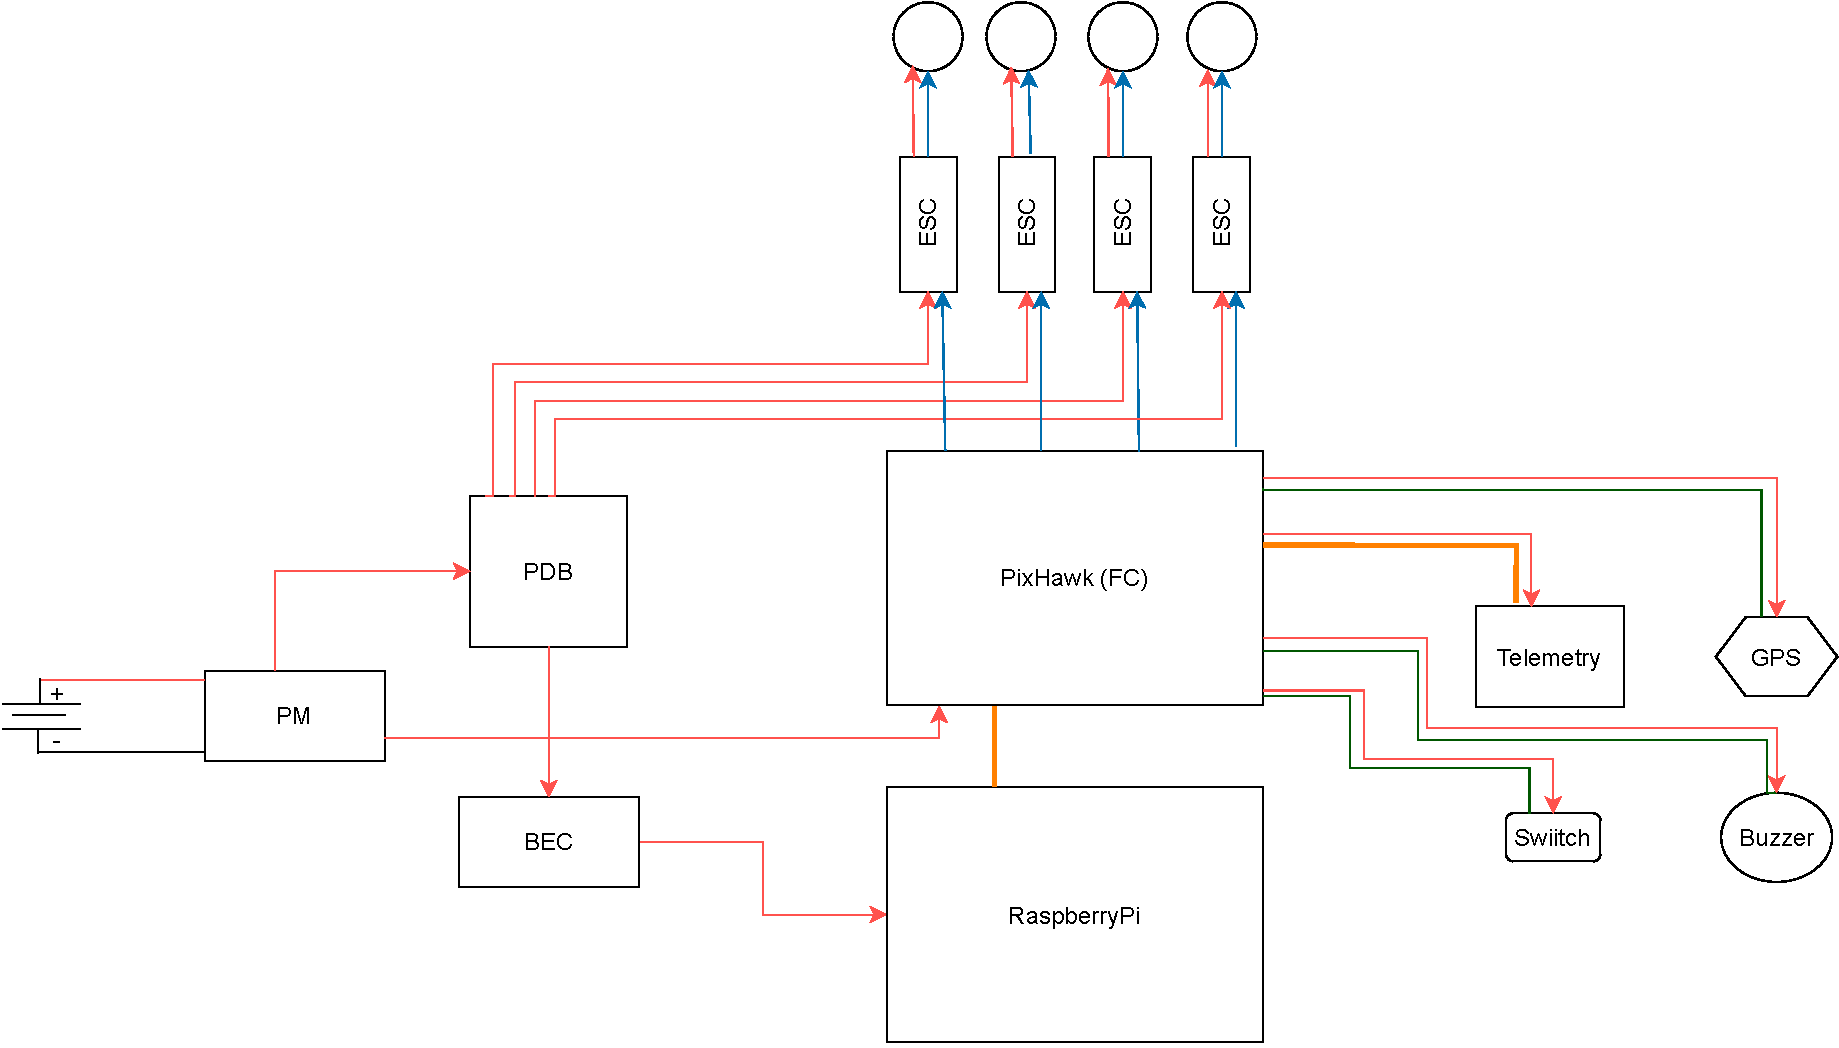
\includegraphics[scale=0.5]{general_wiring.pdf}
    \caption[General Wiring]{General wiring of the hardware setup.\\
    Power connections are labeled red, 
    Blue connections are used for \ac{PWM} signals, 
    Green connections are serial connections, 
    orange connections are more specifically serial UART connections.}
    \label{fig:4_general_wiring}
\end{figure}
\FloatBarrier
\noindent This results in some challenges in providing the correct voltage for
each connected device.
In the current setup this task is taken over by three devices.
The \ac{PM} is directly connected to the battery.
It transfers the battery's voltage to the \ac{PDB} and a lower 5V voltage to
the PixHawk flight controller.
The \ac{PDB} itself is a parallel circuit, thus providing the same voltage
(battery voltage) to each output.
The third device is a \ac{BEC} which is directly connected
to the \ac{PDB} and delivers a constant 5V output.
This can be used to power a companion computer such as a RaspberryPi.\\
All other required peripherals are powered by the PixHawk flight controller
itself.
The main peripherals used in this project are a telemetry module which is used
for communication with a ground station and a \ac{GPS} module used for
improving the drones capabilities to follow a defined trajectory, which is
specifically useful for auto-return~and landing features.
Two more peripherals, a buzzer to output audio warning signals and a manual
kill switch which can immediately stop all four motors, are installed mainly
for safety reasons.\\
The hardware components that actually control the motor rotation speeds,
the \acp{ESC}, are connected to the \ac{PDB} for power supply as well as to
the flight controller that calculates the correct rotation speeds based on the
wanted flight maneuvers and outputs a \ac{PWM} signal for each motor.\\
The presented overall wiring is rather complex but allows relying on one power
source only instead of using multiple power sources for flight hardware and
control hardware including peripherals respectively.

\subsection*{Communication between components}\label{subsec:4_comm}
The drone setup needs hardware components to communicate with each other in 
order to transfer control signals from either the companion computer or from
the ground station to the flight controller.
Even if both options origin from different sources, they use the same
device-to-device communication protocol.
The protocol used for this purpose is the \textit{UART} protocol, which is
acronym for universal asynchronous receiver / transmitter protocol.
It is based on a serial, full duplex connection using six connections.
The connection layout is shown in \autoref{fig:4_uart_wiring},
\begin{figure}[!h]
    \centering
    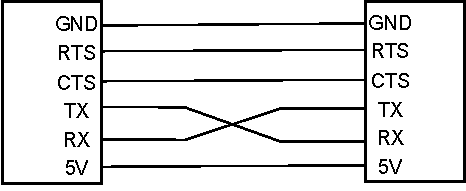
\includegraphics[scale=0.8]{uart_wiring.pdf}
    \caption[UART wiring]{UART wiring}
    \label{fig:4_uart_wiring}
\end{figure}
\FloatBarrier
\noindent where RTS / CTS denote Ready to send and Clear to send.
RX / TX represent the actual data receiving and sending connections
respectively.\\

\noindent UART transfers data using data frames with minimal overhead.
A typical UART frame consists of just a start bit, data bits, a parity bit and
a stop bit.
\autoref{fig:4_uart_frame} visualizes such a data frame. 
\begin{figure}[!h]
    \centering
    
\includegraphics[scale=0.8]{uart_frame.pdf}
    \caption[UART data frame]{Exmple of an UART data frame. The blue marked
    area is the actual data part that is transmitted.}
    \label{fig:4_uart_frame}
\end{figure}
\FloatBarrier
\noindent The shown UART data frame includes 5 data bits, however, the amount
can vary between 5 and 9.
Moreover, the included even parity bit is optional.
The idle state is set to a voltage that represents HIGH level on purpose, so
that any connection failure is easily detectable.
UART can work with any voltages to denote HIGH and LOW levels.
In the quadcopter setup HIGH is represented by 5V and LOW by GND.

    \include{chapter/5_chapt_ergebnis.tex}

    %----- BIBLIOGRAPHY -----
    \pagenumbering{Roman}
    \setcounter{page}{7}
    \cleardoublepage
    \printbibliography[heading=bibintoc, title = {Bibliography}]

    % \appendix
    % \graphicspath{{./figures/}}
\chapter*{Appendix}
\addcontentsline{toc}{chapter}{Appendix}
\renewcommand{\thesection}{\Alph{section}}

\section{Drone}
\label{sec:appendix_drone}
\begin{figure}[htbp]
    \centering
    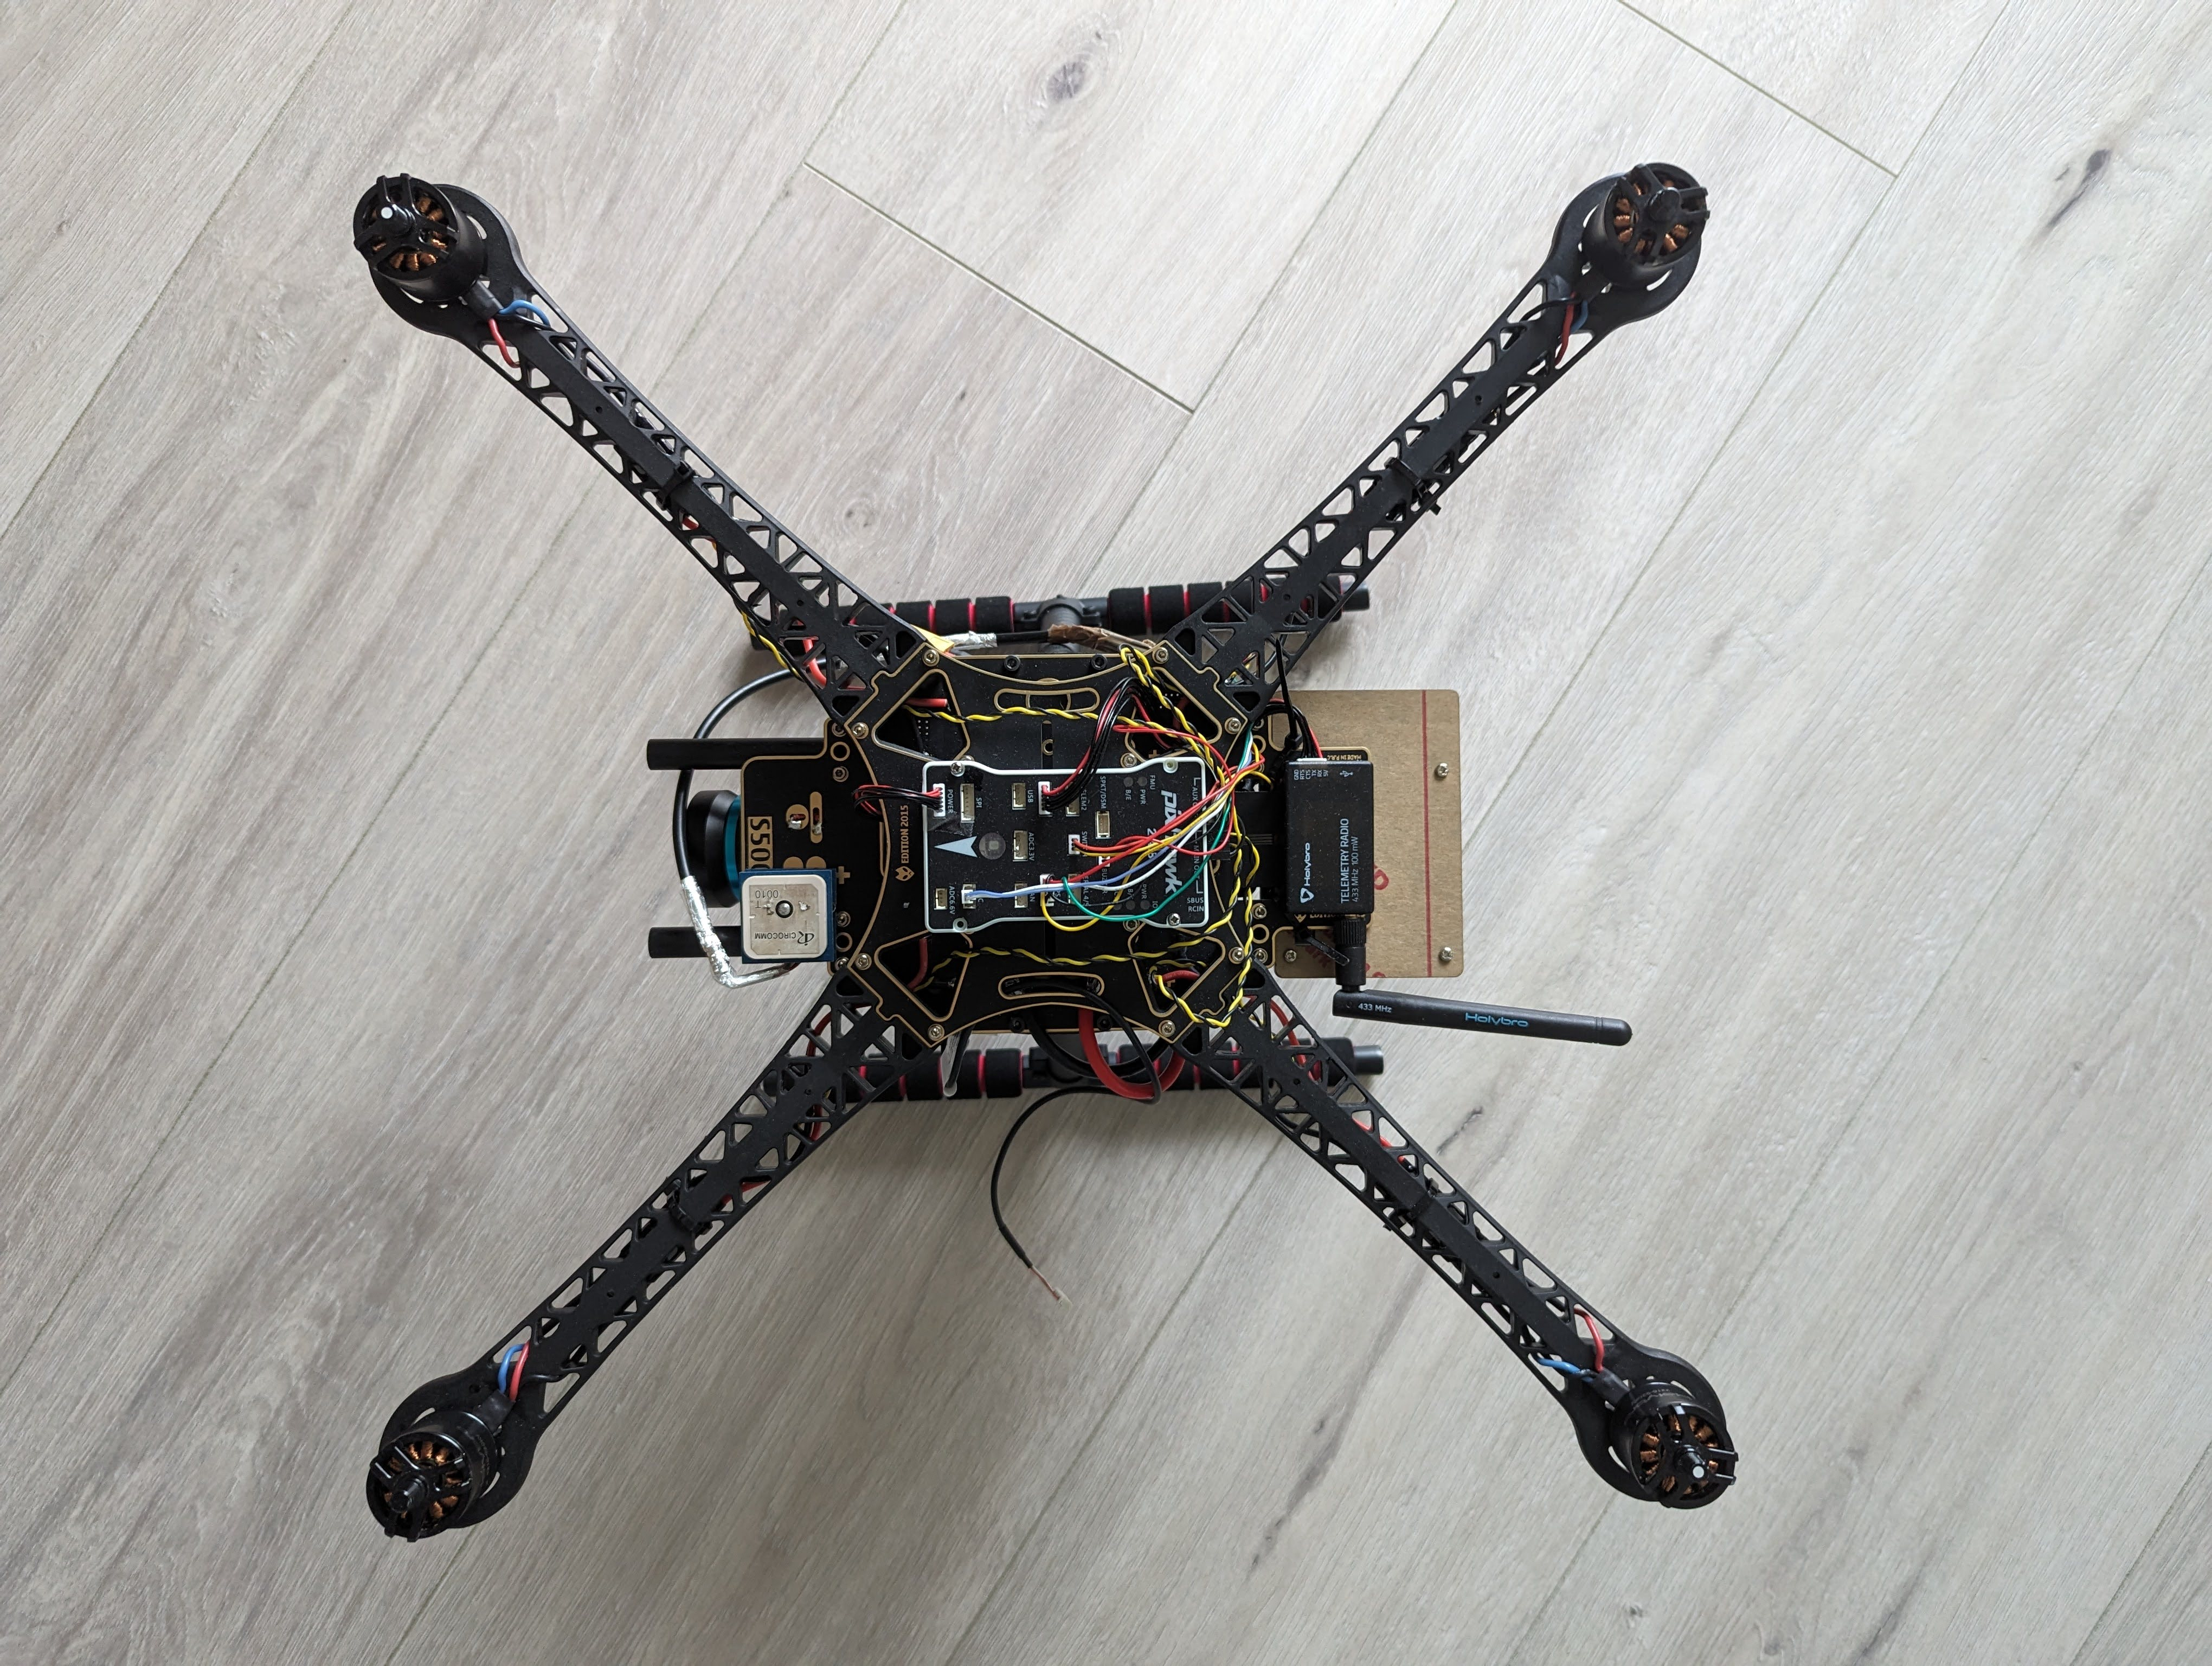
\includegraphics[width=0.4\textwidth]{drone_fully_top.jpg}
    \caption[Fully equipped drone]{Fully equipped drone - Top view.\\
    The PixHawk flight controller is on top of the drone.}
\end{figure}

\begin{figure}[htbp]
    \centering
    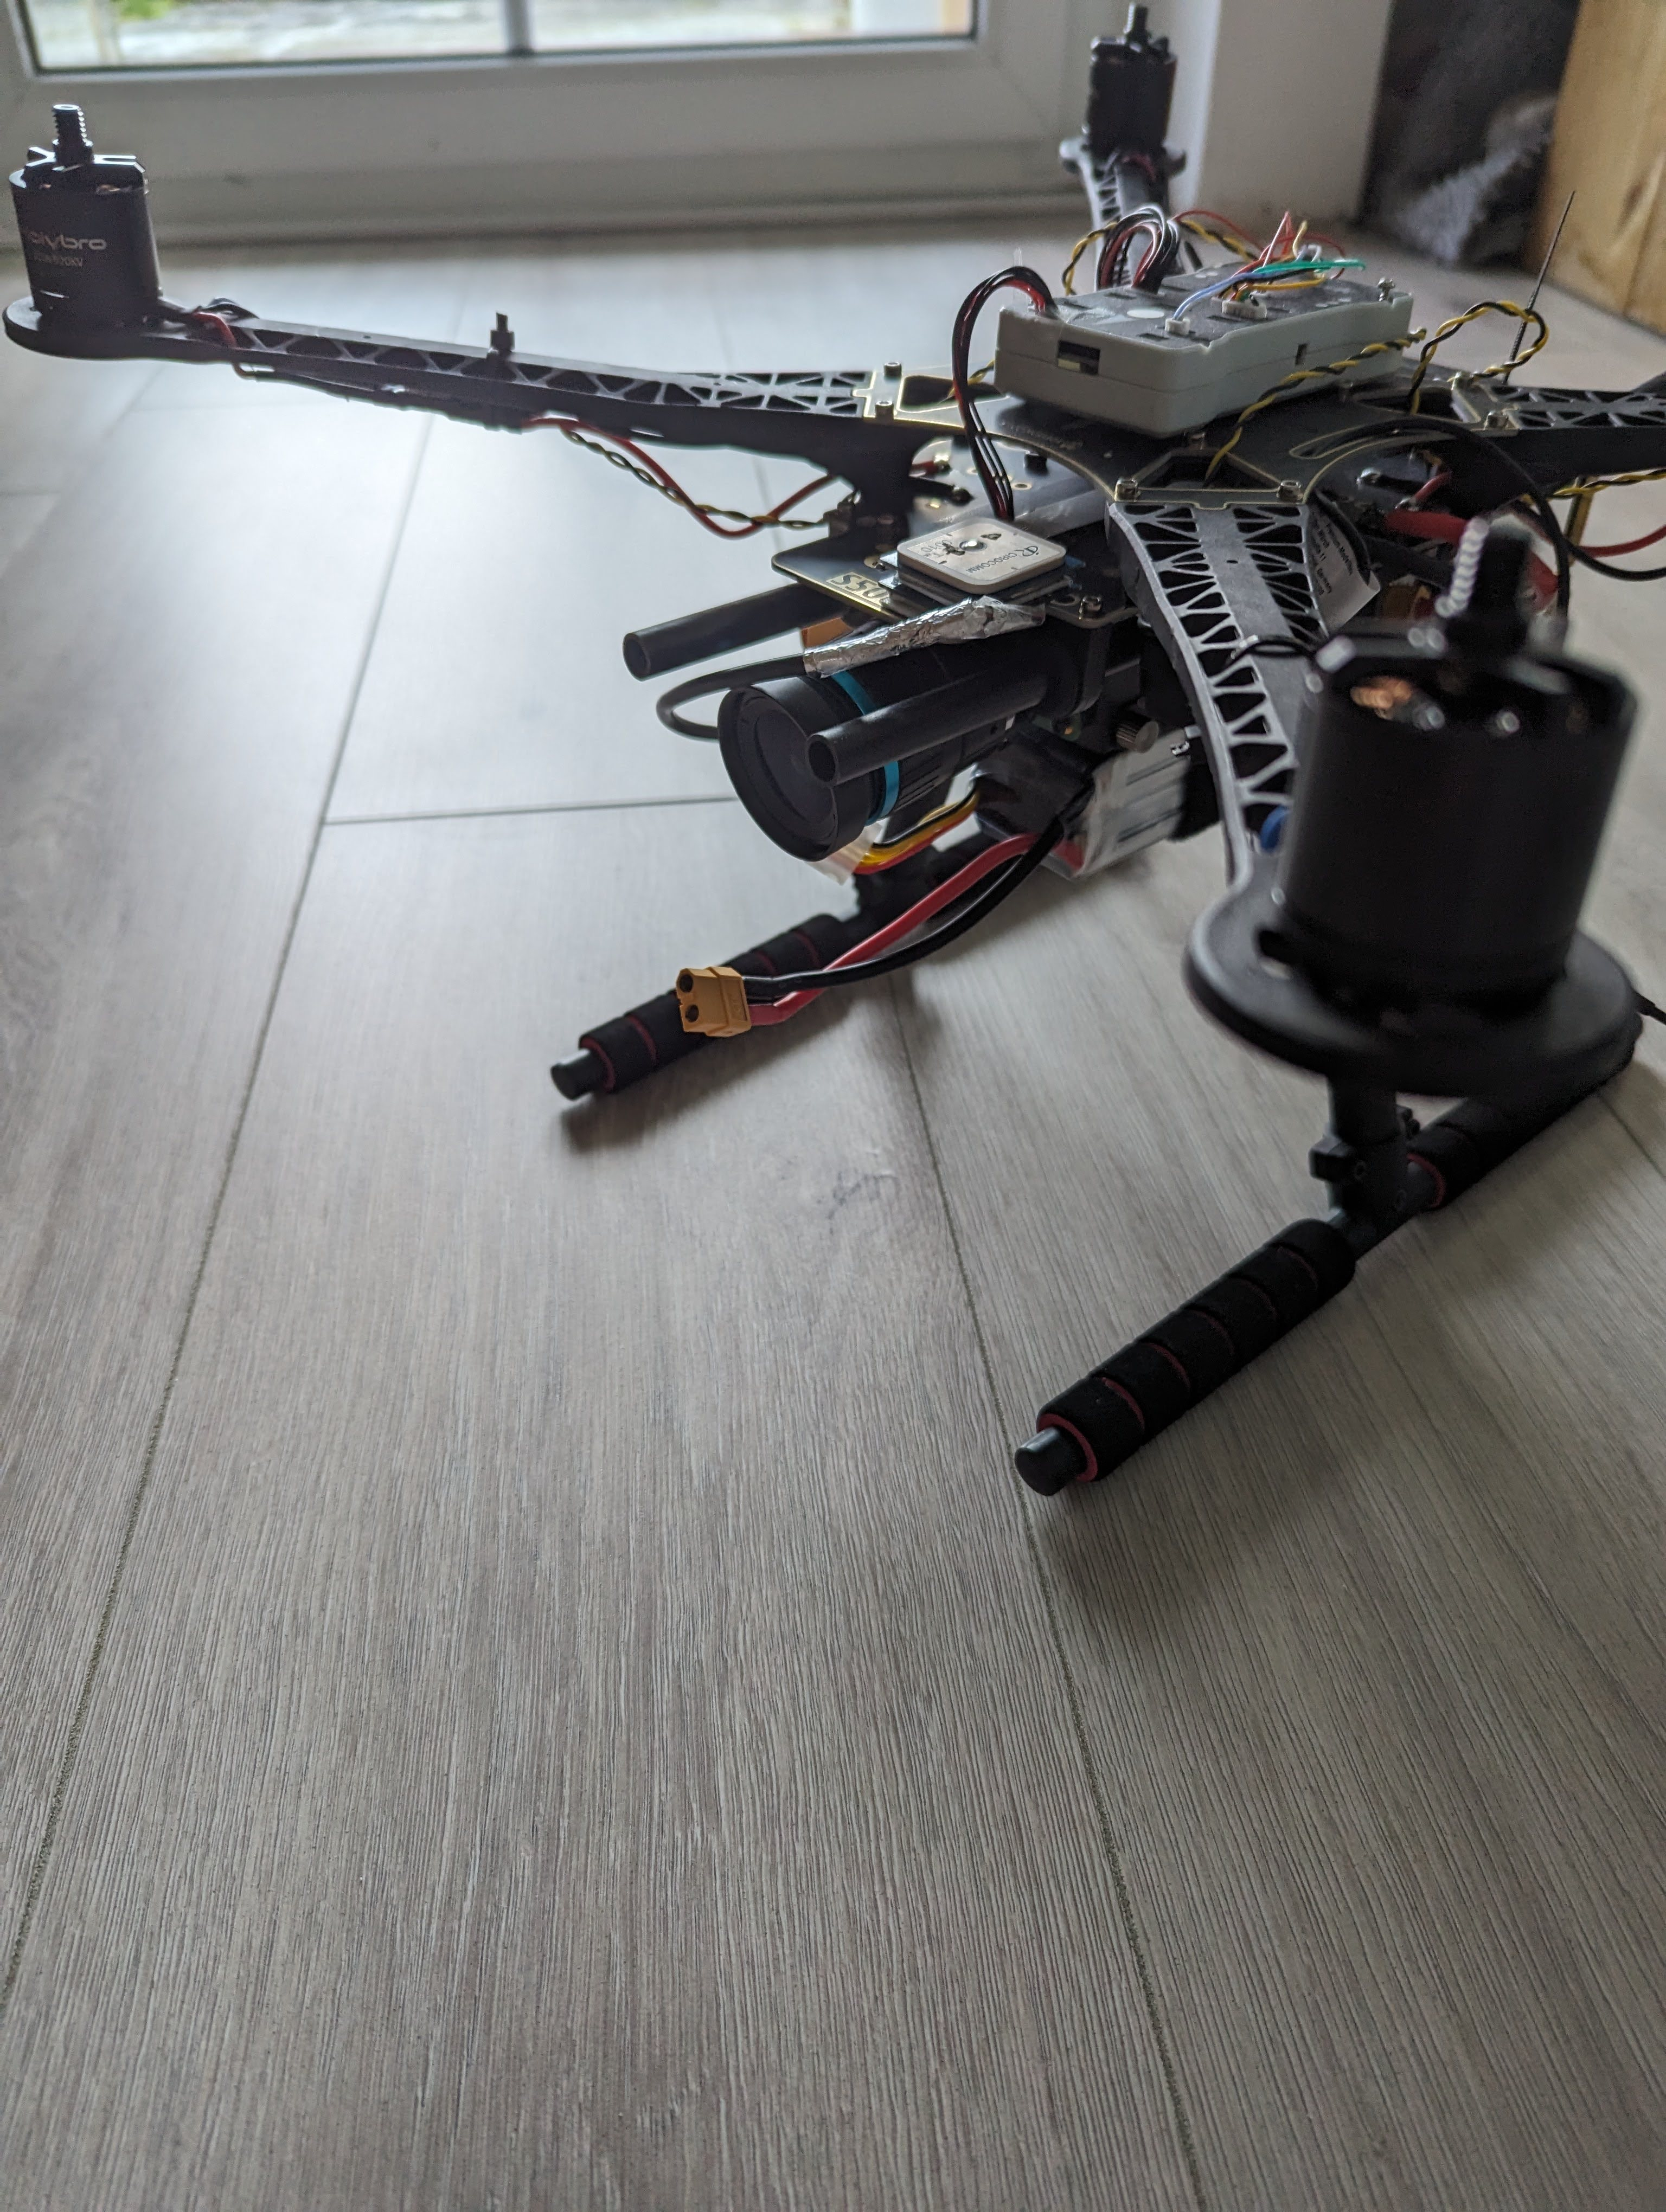
\includegraphics[width=0.4\textwidth]{drone_cam.jpg}
    \caption[Drone with camera]{Drone with a RaspberryPi camera mounted.\\}
\end{figure}
\FloatBarrier
\newpage

\section{Analysis module overview}
\label{sec:appendix_ljanalizer}

The long-jump analysis is implemented as own python module \texttt{ljanalyzer}
with several sub-modules.
The module's structure is showed in the following:
\begin{figure}[h!]
    \centering
    \scalebox{1.2}{ % Adjust the scaling factor as needed
    \centering
        \begin{minipage}{1.0\textwidth}
            \dirtree{%
            .1 ljanalizer.
            .2 Frame.
            .2 Video.
            .2 Posedetector.
            .2 Framebuffer.
            .2 Evaluation.
            .2 Parameterfile.
        }
        \end{minipage}
    }
    \caption[Python analysis module overview]{Python long jump analysis module
    overview.}
    \label{fig:appendix_ljanalizer_overview}
\end{figure}
\FloatBarrier
\noindent As the frame and video sub-module are most important in this work,
both class diagrams are shown in the following:
\begin{figure}[htpb]
    \centering
    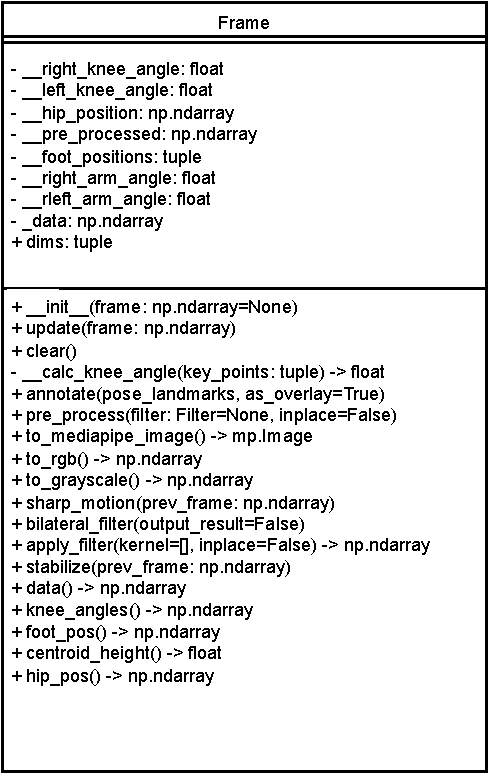
\includegraphics[scale=0.9]{frame_class.pdf}
    \caption[Frame class diagram]{Frame class diagram}
    \label{fig:appendix_frame_class}
\end{figure}

\begin{figure}[htpb]
    \centering
    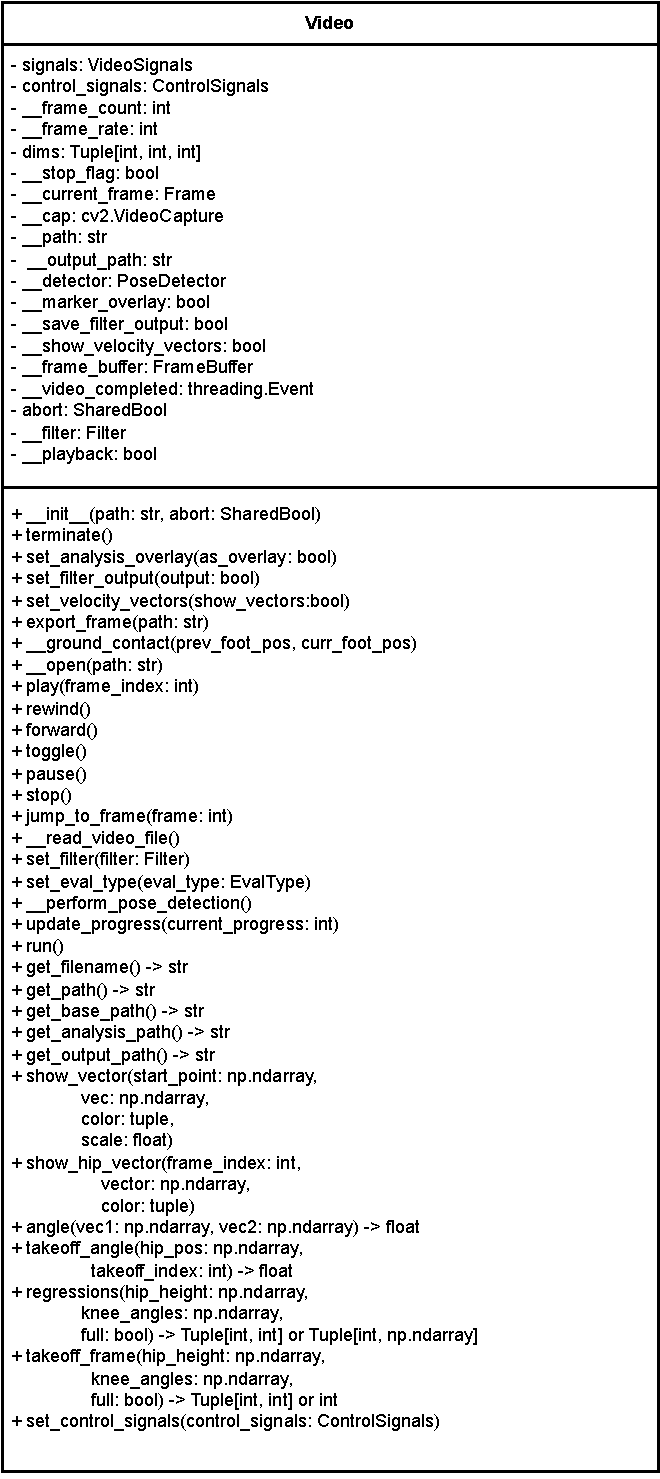
\includegraphics[scale=0.8]{video_class.pdf}
    \caption[Video class diagram]{Video class diagram}
    \label{fig:appendix_video_class}
\end{figure}

\newpage

\section{Live-Stream video visualization}
\label{sec:appendix_livestream}
\begin{figure}[htpb]
    \centering
    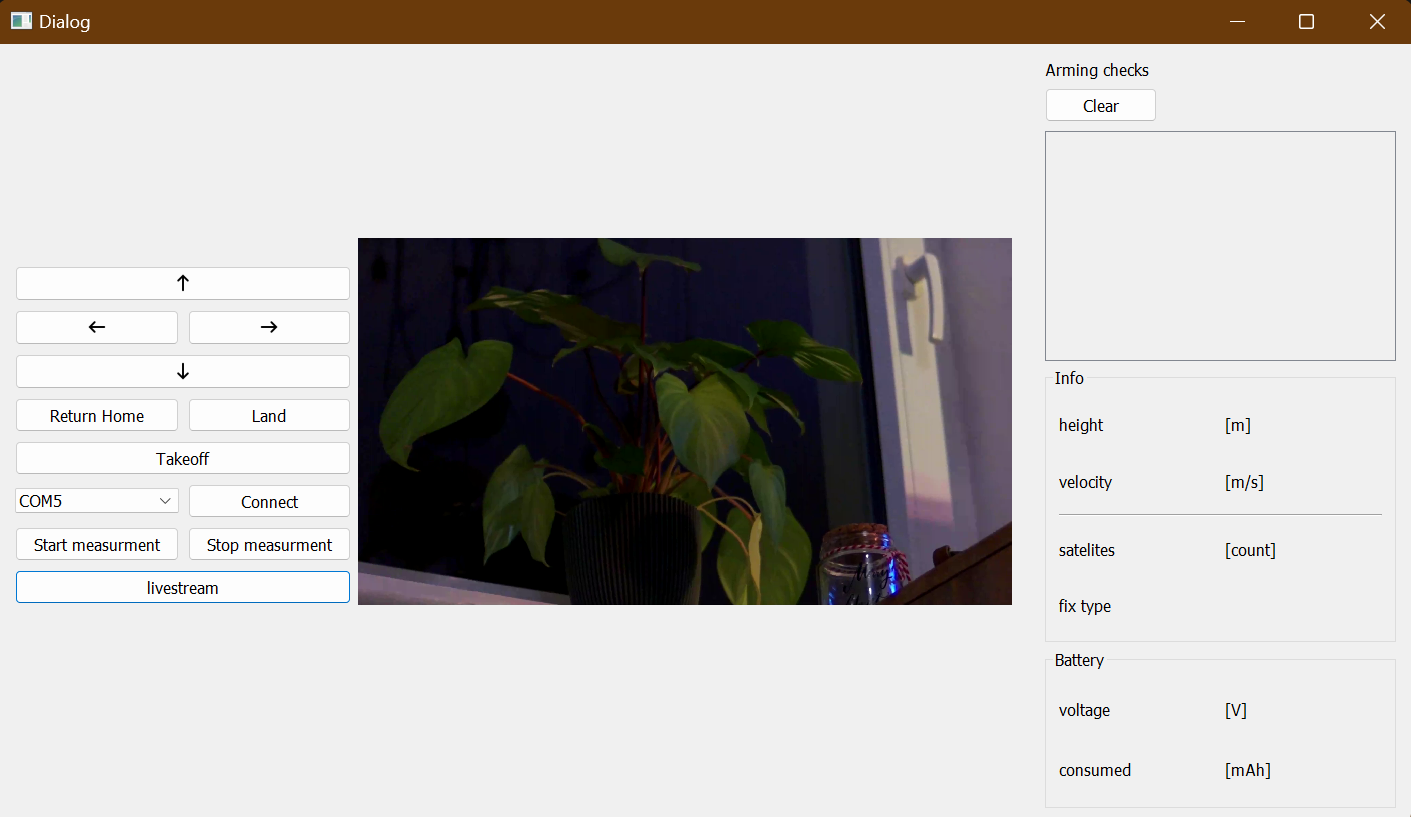
\includegraphics[scale=0.5]{drone_control_panel_live_stream.png}
    \caption[Video Live-stream visualization]{Video Live-stream visualization
    inside the control panel.}
    \label{fig:4_control_panel_live_stream}
\end{figure}

\end{document}